\part{Approches générales stylométriques}

\chapter{Approche supervisé}

\section{Les Machines à vecteurs de support (SVM)}

Le terme de machines à vecteur de support se rapportent à un groupe d'algorithmes de classification basé sur l'apprentissage supervisé \footcites{noauthor_machine_2023}. 
Les SVM ont été largement utilisées dans divers domaines, y compris la classification de textes. Leur flexibilité pour traiter à la fois des séparations linéaires et non linéaires, ainsi que leur capacité à gérer des ensembles de données complexes avec de nombreuses dimensions, en font des outils puissants pour la classification et la régression dans le domaine de l'apprentissage automatique.
Les fondements des SVM ont été posés dans les travaux de Vladimir Vapnik et Alexey Chervonenkis des années 1960, qui ont développé la théorie de la dimension de Vapnik-Chervonenkis (VC-dimension). Cette théorie a permit à Vapnik avec son collègue Corinna Cortes, de formuler le concept de SVM dans les années 1990\footcites{cortes_support-vector_1995}. Leur objectif était de développer un algorithme d'apprentissage automatique capable de gérer des problèmes de classification complexes, notamment ceux impliquant des données non linéairement séparables. Ils ont introduit la notion d'hyperplan de marge maximale et ont développé des méthodes pour résoudre efficacement ce problème d'optimisation. Depuis les SVM ont rapidement gagné en popularité en tant qu'approche puissante pour la classification et la régression. Différentes variantes des SVM coexistent, y compris par l'utilisation de noyaux non linéaires pour traiter des données non séparables linéairement. Cela a conduit au développement de noyaux tels que le noyau gaussien (RBF) et le noyau polynomial qui ne nous intéresse pas particulièrement pour notre cas d'étude.

Depuis les années 2000, les SVM ont continué à évoluer avec l'avancée de la recherche en apprentissage automatique et en traitement du signal. Des variantes plus sophistiquées ont été développées pour aborder des tâches plus complexes, et des extensions ont été proposées pour la classification multi-classes et la régression. Malgré la concurrence qui existent avec de nouvelles approches, les SVM restent pertinentes et sont toujours utilisées pour des tâches de classification et de régression, en particulier lorsque les données sont en nombre limité ou lorsque l'interprétabilité du modèle est nécéssaire. Ils continuent de fournir une base théorique solide pour la compréhension de la complexité de l'apprentissage automatique et de la séparation des données. Les SVM comme classifieur de texte sont donc un choix judicieux du fait qu'ils gèrent facilement un très large nombre de dimensions, ce qui se produit avec une approche en n-grams de features.
Le choix de cet approche se trouve complémentaire des approches que nous déploierons ensuite au sens où, mise à part les choix du type de \textit{features} à extraire et la sélection des hyperparamètres de la SVM, l'ensemble ne dépend pas d'hypothèses inductives. C'est l'algorithme qui sélectionne de manière optimale les objets les plus discriminants pour définir nos classes génériques. En cela, il offre une entrée objectif pour définir des caractéristiques propres aux textes pamphlétaires.


En partant de données étiquetées en différentes classes, l'algorithme SVM cherche à maximiser des frontières entre chacune des classes fournies. Les SVM parviennent à accomplir cette tâche en exploitant des concepts géométriques et mathématiques. L'objectif principal est de trouver un hyperplan dans un espace de plusieurs dimensions. Cet hyperplan peut être linéaire (une simple ligne dans un espace bidimensionnel), mais les SVM peuvent également utiliser des fonctions de noyau pour projeter les données dans des espaces de dimensions supérieures, permettant ainsi de capturer des séparations non linéaires, ce qui est souvent le cas de données textuelles. Cette transformation permet aux SVM de gérer des problèmes de classification complexes et hautement dimensionnels. La notion de \enquote{marge} est cruciale dans les SVM. La marge est la distance entre l'hyperplan et les exemples de données les plus proches de chaque côté. L'objectif est de maximiser cette marge tout en minimisant les erreurs de classification. Les exemples de données qui se trouvent à la limite de la marge, et qui ont un impact sur la position de l'hyperplan, sont appelés \enquote{vecteurs de support}. Ce sont eux qui déterminent la position optimale de l'hyperplan en cherchant à maximiser la marge. 
Il est important de noter que les SVM peuvent également rencontrer des situations où les données ne peuvent pas être parfaitement séparées par un hyperplan. Dans ce cas, la SVM cherche un compromis en introduisant des marges d'erreur, ce qui est souvent désigné par le terme de \enquote{marges souples} (soft margins). Cela permet au modèle d'accepter un certain niveau d'erreur de classification tout en visant toujours à maximiser la marge.

\section{Méthode choisie}

Nous utilisons une implémentation de SVM déployée par Jean-Bapiste Camps nommée SuperStyl\footcites{camps_supervised_2021}. L'avantage de ce choix est de pouvoir facilement effectuer différentes variantes d'extraction de \textit{features} ainsi que différents entraînements en changeant aisément de paramètres et d'hyperparamètres.

Les SVM prennent en entrée non pas les textes eux-mêmes mais une matrice de caractéristiques issues des textes et de la classe à laquelle se rattache le texte. Ces caractéristiques sont les \textit{features} extraites des textes avec leurs occurrences. Une \textit{feature} dans ce contexte est une unité minimale qui couramment est choisie à l'échelle du caractère ou du mot. Pour évaluer la robustesse et la justesse d'un modèle et pour éviter le sous et le sur apprentissage, les SVM fonctionnent en deux temps, le premier sert à former le modèle et le second à vérifier sur de nouvelles données sa justesse.

Une option \textit{Hold-Out Validation} est de manuellement diviser les données en données d'entraînement et données de test. Les données d'entraînement servant à former le modèle en minisant sur ces données-ci ses erreurs, et les données de tests servants à vérifier la bonne généralisation du modèle de SVM ainsi formé. Le choix de la division du corpus de texte en données d'entraînement et de test étant à la discrétion du chercheur, traditionnellement on réserve entre 40\% et 30\% du corpus en données de test.

Il est possible d'augmenter la robustesse d'un modèle en faisant une \textit{cross validation}, c'est-à-dire une multiplication des entraînement et des tests où chaque donnée se sera retrouvée soit en entraînement soit en test dans une des multiples itérations.
Une autre option de division est le \textit{k-fold cross validation} où pour un nombre k, on divise les données en entraînement et en test k nombre de fois. 

Nous utilisons une autre méthode plus optimale sur nos données appelée \textit{leave-one-out cross validation}, cette méthode itérative va exclure de l'entraînement à chaque itération un texte de l'ensemble du corpus pour le fournir en donnée de test. Ainsi il y a autant d'entraînements et de tests que de texte dans le corpus. Cela correspond à un k-fold ou k est égale au nombre total de texte. L'estimation de la performance du modèle sera calculée par la moyenne des résultats sur les données tests. Cette option très robuste est aussi la plus coûteuse en ressource du fait de l'augmentation linéairement liée de ses itérations par rapport à la taille du corpus. C'est l'option que nous choisissons pour son gain de robustesse.

La première étape est de fournir des données cohérentes à l'algorithme de SVM. Nous passons pour chaque texte d'une chaîne de caractères à une représentation cohérente pour la classification. Le choix du contenu de cette représentation est l'étape d'extractions des \textit{features}. Plusieurs options s'offrent à nous. Nous ferons une extraction de \textit{features} par mots en trigrammes. Nous n'excluons pas des \textit{features} les mots outils \textit{ où stopwords} mais nous excluons la ponctuation ainsi que les caractères non alphabétique. Pour l'entrainement nous utiliserons un noyau linéaire, l'état de l'art en classification de textes avec une SVM considère que c'est le choix le plus approprié\footcites{kowalczyk_linear_2014}.

\chapter{Gestion du corpus pour l'approche supervisé SVM}

\section{Constitution de deux corpus}

Nous allons appliquer une extraction de \textit{features} et un entraînement de SVM sur deux corpus spécifiques. Le premier corpus permet de comparer les pamphlets à un ensemble de genre d'autres auteurs très divers pour vérifier l'aspect générique de nos pamphlets. Le second corpus est établi depuis l'ensemble de la production de nos auteurs pamphlétaire pour vérifier la force du signal générique vis-à-vis du signal autorial.

\subsection{Corpus de pamphlet face à d'autres genres d'autres auteurs}

Ce premier corpus est constitué des pamphlets de nos treize auteurs pamphlétaires mis ensemble avec des textes d'autres auteurs de genre distincts tels des romans, des mémoires et biographies et des nouvelles issus du Corpus ANR Chapitres : 2000romans19e20e constitué par l'unité de recherche THALIM 7172 \footcites{anrchapitres_anrchapitres2000romans19e20e_2022}. Il est constitué de 2033 romans francophones de 1813 au milieu du XX\ieme siècle au format xml:tei. Cette ressource est accessible sur Github\footcites{anrchapitres_anrchapitres2000romans19e20e_2023}, nous l'avons transformé au format plain-text en conservant les méta-données, telles que le genre, auteur et titre lorsque ces informations étaient accessibles.

L'intérêt de soumettre les pamphlets à d'autres genres et d'autres auteurs permet de créer un corpus très homogène et de réduire le signal autorial ou idiolecte en son sein. Il est homogène car nous avons accès à autant de texte que nous voulons depuis la base des 2000romans19e20e, ce qui n'est pas le cas de notre propre corpus de tous les textes (tous genres confondus) de nos pamphlétaires.

Pour constituer un corpus qui a du sens pour la SVM, nous partons de notre propre corpus de textes identifiés comme pamphlet et calculons la somme de mots et de caractères correspondants à cet ensemble. Avec cet étalon, nous sélectionnons aléatoirement dans le corpus ANR Chapitres un certains nombre de romans, de mémoires et biographies et de nouvelles qui respectent l'étalon fixé par le genre du pamphlet. C'est un problème d'optimisation ou nous souhaitons obtenir un nombre optimal de texte par genre respectant la contrainte où la somme de leur mots soit au plus proche de la somme des mots des textes pamphlets. Nous avons produit un code qui utilise la librairie \textit{pulp} en python qui résout ce problème d'optimisation linéaire où l'objectif est de sélectionner un certain nombre de fichiers par genre tout en respectant des contraintes sur la somme des caractéristiques des fichiers sélectionnés pour chaque genre. L'approche d'optimisation utilisée ici permet de choisir les fichiers de manière à maximiser le nombre total de fichiers tout en satisfaisant les contraintes imposées. La \textit{table \ref{'tab:corpus-mix-word'}} montrent cette répartition ou le nombre de texte par genre est inégal mais l'étalon de la somme des mots par genre est le plus homogène possible.
\begin{table}[H]
    \centering
    \begin{tabular}{lrrrrr}
    \toprule
    Genre & Nombre de texte & Somme & Min & Max & Moyenne  \\
    \toprule
    \midrule
    roman (ANR Chapitres) & 109 & 2939952 & 681 & 38207 & 26972.03 \\
    \midrule
    mémoire et biographie (ANR Chapitres) & 92 & 2951061 & 1399 & 45185 & 32076.75 \\
    \midrule
    nouvelle (ANR Chapitres) & 141 & 2935918 & 844 & 41442 & 20822.11 \\
    \midrule
    pamphlet & 48 & 2931562 & 2356 & 263090 & 61074.20 \\
    \bottomrule
    \end{tabular}
    \caption{Corpus 1 par genre et par proportion de mots}
    \label{'tab:corpus-mix-word'}
\end{table}

 Sur ce premier corpus constitué nous effectuons un échantillonage par 10000 mots pour obtenir un corpus homogène au niveau de la moyenne de mots par texte par genre. Nous choisissons ce pas de 10000 car il correspond plus au moins au dixième-vingtième des moyenne par texte par genre, ce qui nous assure d'un nombre d'échantillon élevé mais non trop copieux en ressource pour l'entraînement. La \textit{table \ref{'tab:corpus-mix-echantillons-word'}} vous présentent le résultat de cet échantillonnage. Nous remarquons que chaque moyenne par genre de la longueur des textes par mots est homogénéisée grâce à la division des textes en échantillons de 10000 mots, la conséquence évidente est l'augmentation du nombre de \textit{textes} par genre représentant des fractions de 10000 mots de chacun des textes précédents.

\begin{table}[H]
    \centering
    \begin{tabular}{lrrrrr}
    \toprule
    Genre & Nombre de texte & Somme & Min & Max & Moyenne  \\
    \toprule
    \midrule
    roman & 243 & 2939952 & 681 & 19819 & 12098.56 \\
    \midrule
    mémoire et biographie & 256 & 2951061 & 1399 & 19988 & 11527.58 \\
    \midrule
    nouvelle & 272 & 2935918 & 844 & 19984 & 10793.81 \\
    \midrule
    pamphlet & 277 & 2931562 & 2356 & 19970 & 10583.25 \\
    \bottomrule
    \end{tabular}
    \caption{Corpus 1 échantillonné par genre et par proportion de mots}
    \label{'tab:corpus-mix-echantillons-word'}
\end{table}

C'est ce corpus nouvellement constitué le plus homogène possible que nous appliquerons l'extraction des \textit{features}. Nous choisissons d'appliquer une extraction par unigramme de mots. Nous entraînons la SVM avec un noyau LinearSVC en cross-validation Leave-one-out avec le paramètre class-weights bien que le corpus nouvellement constitué soit particulièrement homogène.

\subsection{Corpus uniquement composé de différents genres des auteurs pamphlétaires}

Le second corpus est simplement l'ensemble des textes de nos pamphlétaires classés par genre ou grands ensembles génériques tel que des essais, des pamphlets, des mémoires et biographies, des articles et des romans, la \textit{table \ref{'tab:corpus-word'}} présente de la même manière que pour le corpus précédent la répartition des mots par genre.
L'intérêt du second corpus soumis à la SVM est de vérifier que le signal générique puisse être suffisamment spécifique pour que la SVM identifie le pamphlet comme une classe pertinente de catégorisation malgré un signal autorial fort (tous les textes se divisent alors seulement entre 13 auteurs). Et cela alors que nous sommes limité par notre corpus en nombre de textes par genre, ce qui rend se corpus bien moins homogène que le premier.
Il n'est pas possible d'espérer uniformiser la somme des mots par genre dans ce cas présent car nous ne souhaitons pas exclure des textes pour y parvenir étant donné qu'ils représentent l'ensemble des textes que nous avons réussi à identifier de nos auteurs pamphlétaires.

\begin{table}[H]
    \centering
    \begin{tabular}{lrrrrr}
    \toprule
    Genre & Nombre de texte & Somme & Min & Max & Moyenne  \\
    \toprule
    \midrule
    roman & 78 & 5702861 & 1450 & 284630 & 73113.60 \\
    \midrule
    mémoire et biographie & 13 & 757025 & 6043 & 88988 & 58232.69 \\
    \midrule
    article & 25 & 473482 & 570 & 114731 & 18939.28 \\
    \midrule
    essai & 37 & 2527073 & 2108 & 819600 & 68299.27 \\
    \midrule
    pamphlet & 48 & 2931562 & 2356 & 263090 & 61074.20 \\
    \bottomrule
    \end{tabular}
    \caption{Corpus 2 par genre et par proportion de mots}
    \label{'tab:corpus-word'}
\end{table}

Ce second corpus va lui aussi subir un échantillonage des textes tout les 10000 mots, cela permettra une certaine homogénéisation de la moyenne des mots par texte que l'on peut observer sur la \textit{table \ref{'tab:corpus-mix-echantillons-word'}}. Certaines classes se retrouvent sur représentées mais nous comptons sur l'hyperparamètre class\_weights implémenté dans \textit{Superstyl} pour appliquer un poids à chaque classe permettant de rétablir un équilibrage entre elles.

\begin{table}[H]
    \centering
    \begin{tabular}{lrrrrr}
    \toprule
    Genre & Nombre de texte & Somme & Min & Max & Moyenne  \\
    \toprule
    \midrule
    roman & 542 & 5702861 & 1450 & 19967 & 10521.88 \\
    \midrule
    mémoire et biographie & 70 & 757025 & 6043 & 18988 & 10814.64 \\
    \midrule
    article & 56 & 473482 & 570 & 18900 & 8455.03 \\
    \midrule
    essai & 239 & 2527073 & 2108 & 19600 & 10573.52 \\
    \midrule
    pamphlet & 277 & 2931562 & 2356 & 19970 & 10583.25 \\
    \bottomrule
    \end{tabular}
    \caption{Corpus 2 par genre et par proportion de mots}
    \label{'tab:corpus-echantillon-word'}
\end{table}

\section{Résultats et analyse de la SVM sur chacun des corpus}

Pour chacun des deux corpus, la SVM produit des métriques et différentes données propre à indiquer la pertinence de la classification ainsi que les réussites et les échecs des prédictions de chaque texte par classe. La sortie de l'entraînement de \textit{Superstyl}, l'implémentation de la SVM que nous utilisons donne à voir cinq métriques distinctes qui chacune éclaire notre compréhension de la pertinence du classifieur sur nos données. Ces métriques sont prédéfinies au sens de l'implémentation de \textit{SuperStyl}.

Précision :\\
La précision mesure la proportion de prédictions positives faites correctement par le modèle parmi toutes les prédictions positives qu'il a effectuées. Une haute précision indique que le modèle a tendance à être prudent lorsqu'il prédit l'appartenance d'un texte à une classe.

\begin{equation}
Pr\acute{e}cision = \frac{Vrais Positifs}{Vrais Positifs + Faux Positifs}
\end{equation}

Rappel (ou Sensibilité) :\\
Le rappel mesure la proportion de prédictions positives correctes parmi toutes les instances réellement positives. Un rappel élevé indique que le modèle a la capacité de détecter la plupart des textes appartenant à une classe.

\begin{equation}
Rappel = \frac{Vrais Positifs}{Vrais Positifs + Faux N\acute{e}gatifs}
\end{equation}

F1-score :\\
Le F1-score est une métrique qui combine à la fois la précision et le rappel en une seule valeur. Cela est particulièrement utile lorsque qu'il faut équilibrer la précision et le rappel, car ces deux mesures peuvent être en conflit. Le F1-score est la moyenne harmonique de la précision et du rappel, ce qui permet de donner plus de poids aux valeurs basses. Un F1-score élevé indique un bon équilibre entre la précision et le rappel.

\begin{equation}
F1-score = \frac{2 \times (Pr\acute{e}cision \times Rappel)}{Pr\acute{e}cision + Rappel}
\end{equation}

Accuracy (Précision globale) :\\
L'accuracy mesure la proportion de prédictions correctes (positives et négatives) faites par le modèle parmi toutes les prédictions. C'est la métrique la plus simple, mais elle peut être trompeuse lorsque les classes sont déséquilibrées. Par exemple, si nous avons une classe très majoritaire, un modèle prédisant toujours cette classe obtiendra une bonne \textit{accuracy} même s'il ne prédit jamais l'autre classe.

\begin{equation}
Accuracy = \frac{Vrais Positifs + Vrais N\acute{e}gatifs}{Total\quad des\quad instances}
\end{equation}

Macro-Average :\\
Le macro-average est une métriques pour calculer des mesures comme la précision, le rappel et le F1-score de l'ensemble de nos classes. C'est la moyenne non pondérée sur toutes les classes pour une métrique donnée. Cela garantit que chaque classe est traitée avec la même importance, indépendamment de sa taille.

\begin{equation}
Macro-Average = \frac{\sum_{chaque\quad classe} (M\acute{e}trique\quad pour\quad la\quad classe)}{Nombre\quad total\quad de\quad classes}
\end{equation}


Weighted-Average :\\
 Contrairement au macro-average, le weighted-average prend en compte le déséquilibre des classes. Il calcule la moyenne des métriques en fonction de la distribution des classes. Les classes avec plus d'instances ont un poids plus élevé dans le calcul de la moyenne, tandis que les classes moins représentées ont un poids plus faible.

\begin{equation}
Weighted-Average = \frac{\sum_{chaque\quad classe} (M\acute{e}trique\quad de\quad la\quad classe \times Poids\quad de\quad la\quad classe)}{Nombre\quad total\quad d'instances}
\end{equation}

En plus de ces métriques nous pouvons analyser la matrice de confusion indiquant le nombre de texte par classes véridiques et par classes prédites. Mais aussi le tableau des textes mal attribués avec leur classe réelle et leur classe prédite. Et enfin un diagramme à barres par des classes indiquant les \textit{features} significatives et leur coefficients. L'ensemble de ces métriques, tableaux et graphiques permettent au mieux de comprendre la pertinence et la robustesse du classifieur.

\subsection{Sortie du Corpus 1}
Pour notre corpus de texte issu de l'ANR Chapitres et de notre ensemble de textes pamphlétaires, nous constatons que le genre du pamphlet est la classe la mieux identifiée. Les métriques générales de l'accuracy, macro-average et weighted average montrent que le modèle produit 20\% d'erreur toutes classes confondues. Nos trois classes roman, mémoire et biographie et nouvelle sont celles qui ont le plus de mal à être identifiée de manière indépendante. Cela tient probablement à leur proximité de champ générique là où la classe pamphlet est pleinement distingué. Sur la \textit{table \ref{'tab:matriceconfusioncorpus1'}} nous constatons que seule deux échantillons de la classe pamphlet sont identifiés comme appartenant à une autre classe, en l'occurrence mémoire et biographie. La table des mauvaises attributions, \textit{table \ref{tab:misattributions-corpus1}}, indique qu'il s'agit du premier échantillon de 10000 mots de \textit{Bagatelles pour un massacre} de Louis-Ferdinand Céline et de \textit{La Noire Idole} de Laurent Tailhade. La première mauvaise attribution est composé du passage de la présentation du premier ballet par le narrateur, \textit{La Naissance d'une fée}. La seconde mauvaise attribution est aussi un cas limite en cela qu'elle porte en elle une grande part de narration de petites histoires sur la prise d'opioïde par les grands du monde. 
D'autres cas limites apparaissent dans les mauvaises attributions tel que des échantillons d'\textit{Aden Arabie} de Paul Nizan qui porte des passages souvent qualifiés de pamphlétaires.

\begin{table}[H]
    \centering 
    \begin{tabular}{l c c c c}
        \toprule
             & precision & recall & f1-score & support \\
        \toprule
        \midrule
        roman & 0.81 & 0.75 & 0.78 & 243 \\
        \midrule
        mémoire et bio. & 0.71 & 0.70 & 0.70 & 256\\
        \midrule
        nouvelle & 0.72 & 0.74 & 0.73 & 272\\
        \midrule
        pamphlet & 0.94 & 0.99 & 0.97 & 277\\
        \midrule
        & & & & \\
        \midrule
        accuracy & & & \textbf{0.80} & 1048 \\
        \midrule
        macro-average & 0.80 & 0.80 & 0.80 & 1048\\
        \midrule
        weighted average & 0.80 & 0.80 & 0.80 & 1048\\

        \bottomrule
    \end{tabular}
\caption{Sortie de la SVM sur corpus 1 échantillonné, 3-mots, LOOCV}
\label{'tab:SVMcorpus1'}
\end{table} 

\begin{table}[H]
    \centering 
    \begin{tabular}{|c|l|c|c|c|c|}
        \hline
        \multicolumn{2}{|c|}{} & \multicolumn{4}{c|}{Prédiction} \\
        \cline{3-6}
        \multicolumn{2}{|c|}{} & roman & mémoire et bio. & nouvelle & pamphlet \\
        \hline
        & roman & 183 & 24 & 34 & 2 \\
        \cline{2-6}
        \multirow{3}*{Vrai} & mémoire et bio. & 22 & 179 & 42 & 13 \\
        \cline{2-6}
        & nouvelle & 22 & 48 & 200 & 2 \\
        \cline{2-6}
        & pamphlet & 0 & 2 & 0 & 275 \\
        \hline
    \end{tabular}
\caption{Matrice de confusion du corpus 1 échantillonné}
\label{'tab:matriceconfusioncorpus1'}
\end{table}
La Matrice de confusion présente dans la \textit{table \ref{'tab:matriceconfusioncorpus1'}} permet d'observer la répartition des erreurs de classification qui est assez homogène entre les classes excepté pour la classe pamphlet où très peu d'échantillons de cette classe se retrouve mal classé et peu d'échantillon d'autres classes se retrouvent classés en pamphlet.

\begin{figure}[H]
\centering %
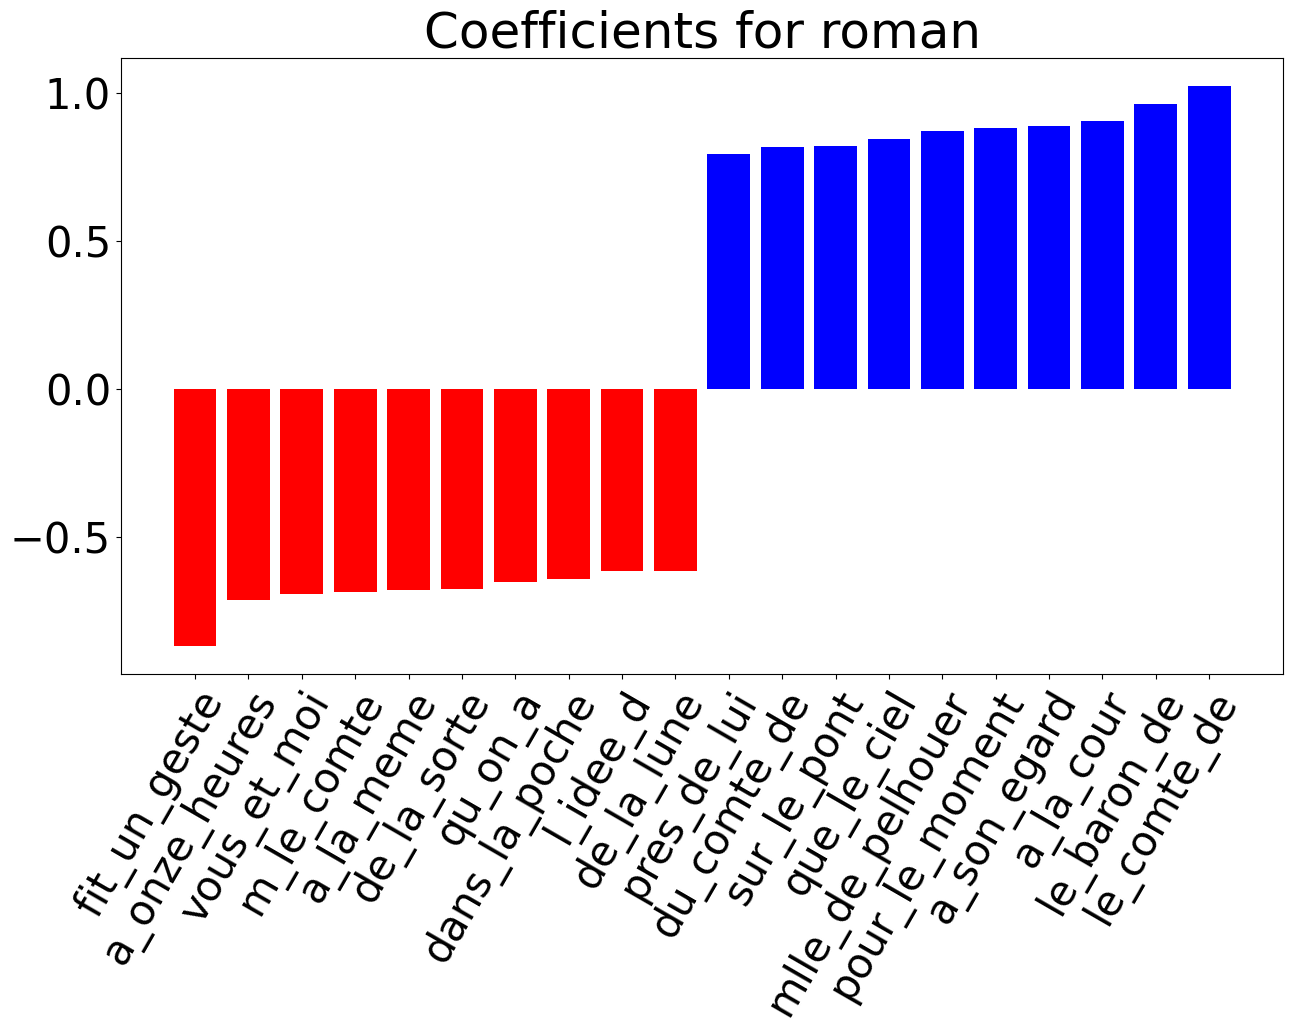
\includegraphics[width=0.70\textwidth]{img/coefs-corpus1-roman.png}
\caption{\textit{Diagramme à barres des coefficients de la classe roman du corpus 1}}
\label{'fig:coefs-corpus1-roman'}
\end{figure}

\begin{figure}[H]
\centering %
\includegraphics[width=0.70\textwidth]{img/coefs-corpus1-mémoire et bio..png}
\caption{\textit{Diagramme à barres des coefficients de la classe mémoire et biographie du corpus 1}}
\label{'fig:coefs-corpus1-mémoire et bio.'}
\end{figure}

\begin{figure}[H]
\centering %
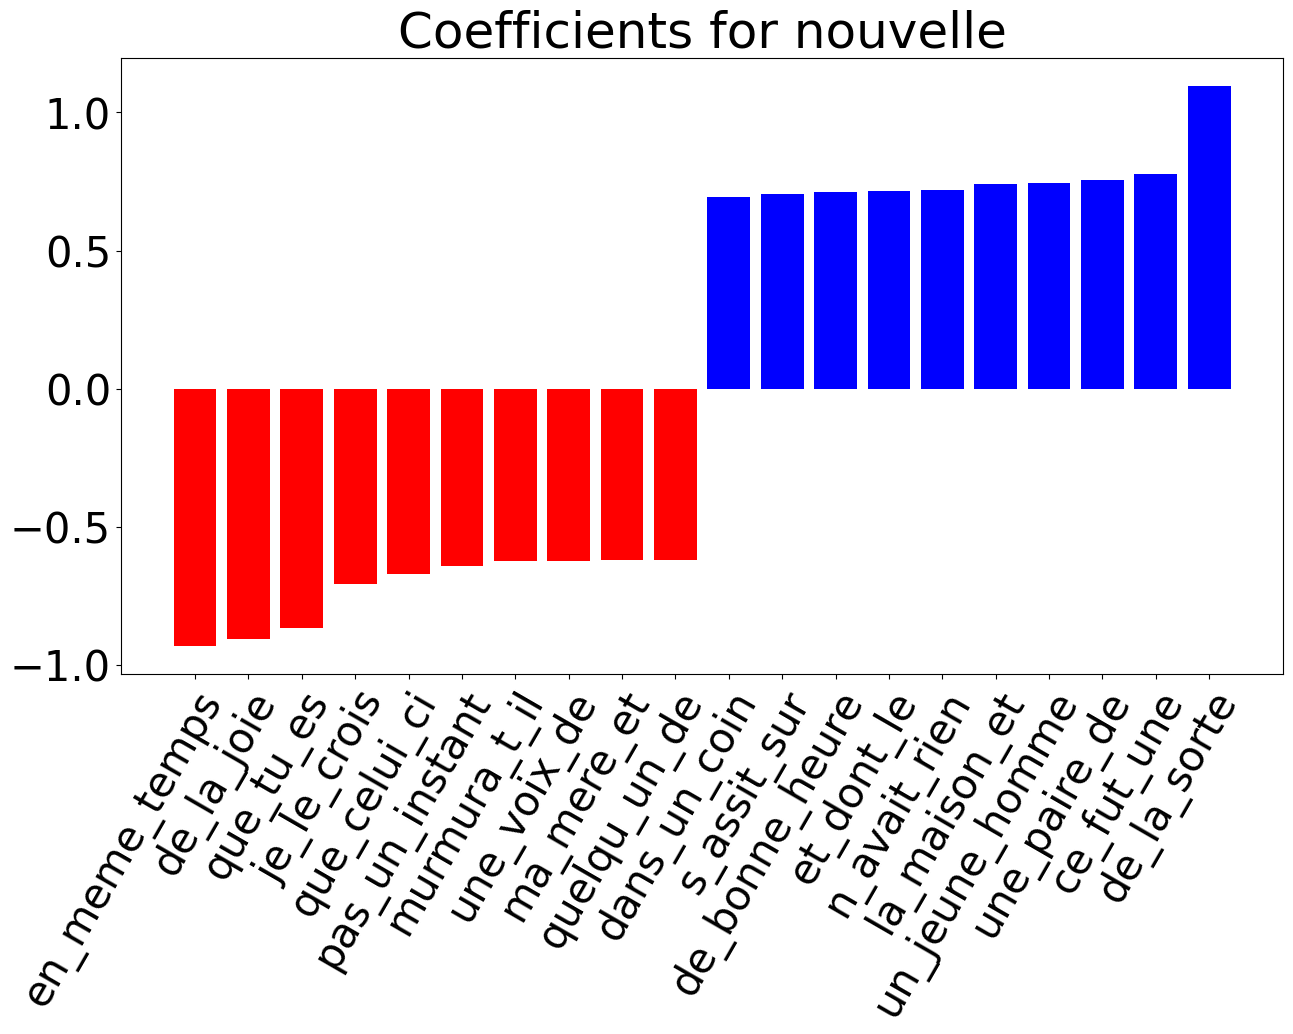
\includegraphics[width=0.70\textwidth]{img/coefs-corpus1-nouvelle.png}
\caption{\textit{Diagramme à barres des coefficients de la classe nouvelle du corpus 1}}
\label{'fig:coefs-corpus1-nouvelle'}
\end{figure}

\begin{figure}[H]
\centering %
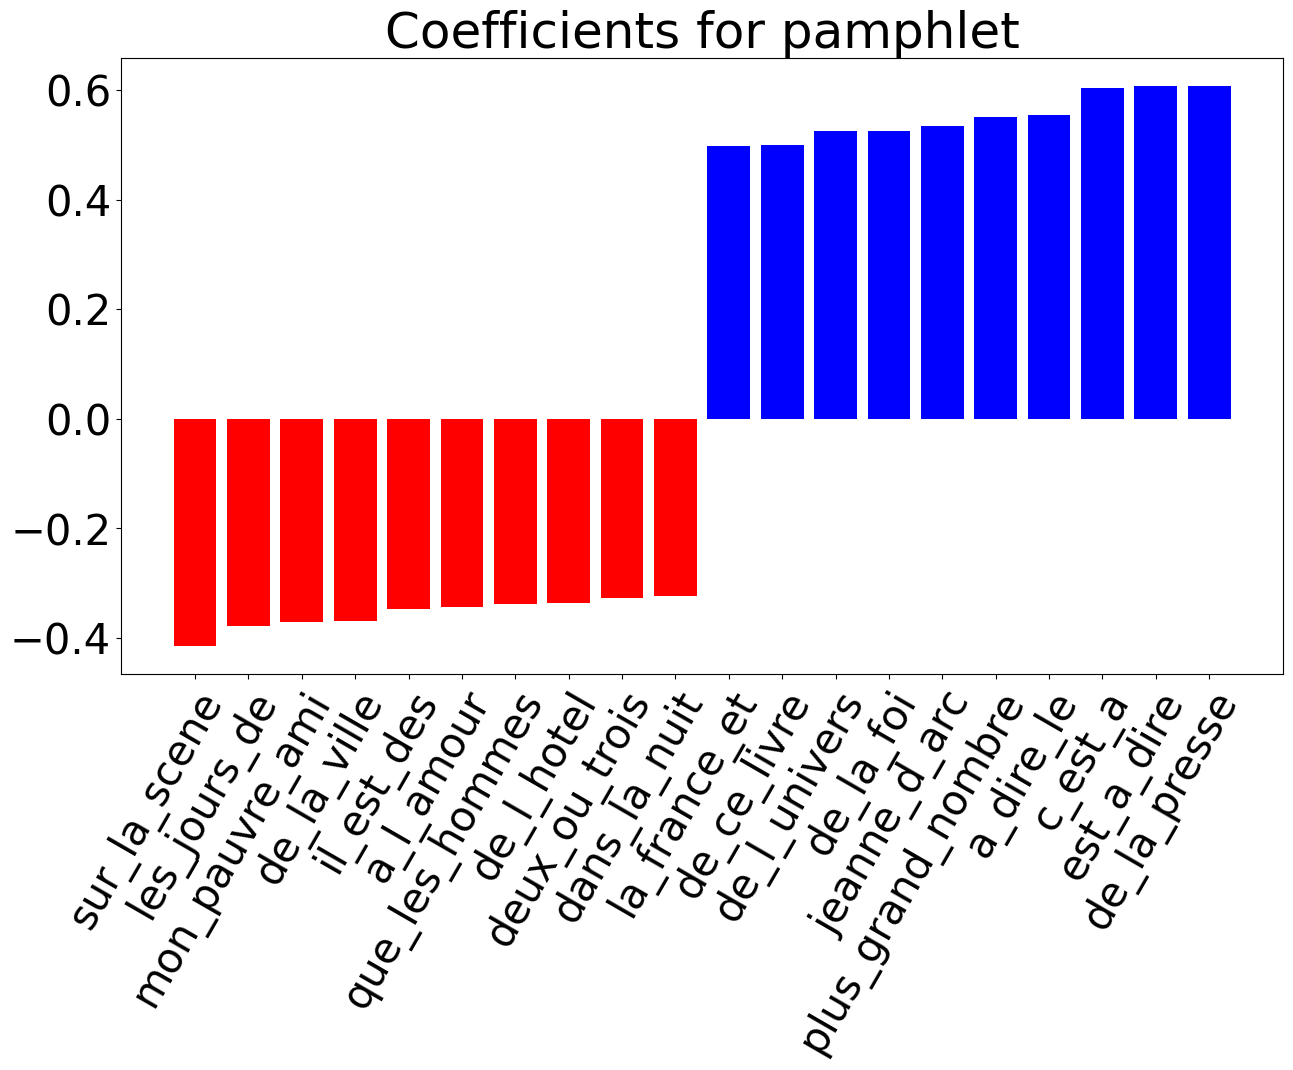
\includegraphics[width=0.70\textwidth]{img/coefs-corpus1-pamphlet.png}
\caption{\textit{Diagramme à barres des coefficients de la classe pamphlet du corpus 1}}
\label{'fig:coefs-corpus1-pamphlet'}
\end{figure}

Au niveau des diagrammes à barres des coefficients des classes du roman, de la nouvelle et des mémoires et biographies, nous pouvons regrouper plusieurs trigrammes de mots en groupes distincts. Le principale problème pour analyser ces fragments de proposition est qu'ils dépendent d'un contexte que nous ne pouvons observer ici. Nous regroupons en un champ générique les trois classes de mémoire et bio., roman et nouvelle en différents type de trigramme. Les trigrammes relatifs à la narration et à la description :
\enquote{\textit{près de lui}} (Roman), \enquote{\textit{sur le pont}} (Roman), \enquote{\textit{pour le moment}} (Roman), \enquote{\textit{dans un coin}} (Nouvelle), \enquote{\textit{s'assit sur}} (Nouvelle), \enquote{\textit{de bonne heure}} (Nouvelle).
Lest trigrammes liés aux personnages et aux titres de noblesse :
\enquote{\textit{mlle de pelhouer}} (Roman), \enquote{\textit{le baron de}} (Roman), \enquote{\textit{le comte de}} (Roman), \enquote{\textit{m le comte}} (Mémoire), \enquote{\textit{un jeune homme}} (Nouvelle), \enquote{\textit{du comte de}} (Roman).
Les trigrammes indiquant une proximité géographique ou spatiale :
\enquote{\textit{dans un coin}} (Nouvelle), \enquote{\textit{s'assit sur}} (Nouvelle), \enquote{\textit{hôtel de ville}} (Mémoire).
Les trigrammes indiquant une heure spécifique ou une durée :
\enquote{\textit{pour le moment}} (Roman), \enquote{\textit{de bonne heure}} (Nouvelle).
Les trigrammes relatifs à la connaissance et à l'expérience personnelle :
\enquote{\textit{tu ne sais}} (Mémoire), \enquote{\textit{il m'était}} (Mémoire).
Un trigramme indiquant des quantités approximatives :
\enquote{\textit{deux ou trois}} (Mémoire).
Un trigramme indiquant une observation ou un événement :
\enquote{\textit{on a vu}} (Mémoire).
Un trigramme exprimant une manière ou un processus :
\enquote{\textit{de la sorte}} (Nouvelle). Pour ces trois classes les trigrammes indiquent bien une réalité générique narrative sous-jacente.

Quand à la classe pamphlet nous divisons les trigrammes en quatre catégories. Les trigrammes liés à des thèmes spécifiques :
\enquote{\textit{la france et}}, \enquote{\textit{de ce livre, de l'univers}}, \enquote{\textit{de la foi}}, \enquote{\textit{jeanne d'arc}}.
Les trigrammes introduisant une déclaration ou une clarification :
\enquote{\textit{à dire le}}, \enquote{\textit{c'est à dire}}.
Un trigramme lié aux médias et à la communication :
\enquote{\textit{de la presse}} et un trigramme indiquant une généralisation ou une quantité :
\enquote{\textit{plus grand nombre}}

Nous espérions trouver dans les trois classes mémoire, roman et nouvelle des verbes d'incises qui distinguassent mieux ce champ générique de celui du pamphlet mais tel n'en fut pas le cas. Nous observons au-delà des thèmes qu'ouvrent les trigrammes, des trigrammes propres à une écriture argumentative, ce qui semble bien distinguer le champ générique de la narration du pamphlet plus proche de l'essai argumentatif. Les thèmes capturés par la SVM pour le pamphlet le distingue bien des autres classes. Il est notable d'observer la présence de Jeanne d'Arc qui est une figure de référence pour la plupart des pamphlétaires mais aussi les enjeux de patriotisme et de religion.




\subsection{sortie du Corpus 2}

Ce second corpus constitué uniquement des textes des auteurs pamphlétaires donne des résultats supérieurs en terme d'accuracy globale, chaque classe étant globalement mieux reconnue (\textit{table \ref{'tab:SVMcorpus2'}}) même si la classe pamphlet a un f1-score légèrement inférieur à celui du premier corpus. Nous sommes particulièrement surpris qu'il y ai une si bonne distinction entre la classe pamphlet et celle de l'essai, leur proximité de champ générique ajouté à la force du style autorial nous laissait à penser qu'ils s'interférassent l'un l'autre plus profondément. C'est la classe article qui donne la moins bonne classification, la principale cause peut être la faiblesse de sa consistance en terme de taille, mais il semble possible que la proximité du signal autorial puisse brouiller la classification.

\begin{table}[H]
    \centering 
    \begin{tabular}{l c c c c}
        \toprule
             & precision & recall & f1-score & support \\
        \toprule
        \midrule
        roman & 0.92 & 0.96 & 0.94 & 542 \\
        \midrule
        mémoire et biographie & 0.94 & 0.86 & 0.90 & 70\\
        \midrule
        article & 0.76 & 0.68 & 0.72 & 56\\
        \midrule
        essai & 0.83 & 0.88 & 0.85 & 239\\
        \midrule
        pamphlet & 0.91 & 0.83 & 0.87 & 277\\
        & & & & \\
        \midrule
        accuracy & & & \textbf{0.89} & 1184 \\
        \midrule
        macro-average & 0.87 & 0.84 & 0.85 & 1184\\
        \midrule
        weighted average & 0.89 & 0.89 & 0.89 & 1184\\

        \bottomrule
    \end{tabular}
\caption{Sortie de la SVM sur corpus 2 échantillonné, 3-mots, LOOCV, class-weight}
\label{'tab:SVMcorpus2'}
\end{table} 

\begin{table}[H]
    \centering 
    \begin{tabular}{|c|l|c|c|c|c|c|}
        \hline
        \multicolumn{2}{|c|}{} & \multicolumn{5}{c|}{Prédiction} \\
        \cline{3-7}
        \multicolumn{2}{|c|}{} & roman & mémoire et bio. & article & essai & pamphlet \\
        \hline
        & roman & 518 & 3 & 1 & 17 & 3 \\
        \cline{2-7}
        \multirow{3}*{Vrai} & mémoire et bio. & 7 & 60 & 1 & 1 & 1 \\
        \cline{2-7}
        & article & 9 & 0 & 38 & 2 & 7 \\
        \cline{2-7}
        & essai & 12 & 0 & 4 & 211 & 12 \\
        \cline{2-7}
        & pamphlet & 16 & 1 & 6 & 24 & 230 \\
        \hline
    \end{tabular}
    \caption{Matrice de confusion du corpus 2 échantillonné}
    \label{'tab:matriceconfusioncorpus2'}
\end{table}

\begin{figure}[H]
\centering %
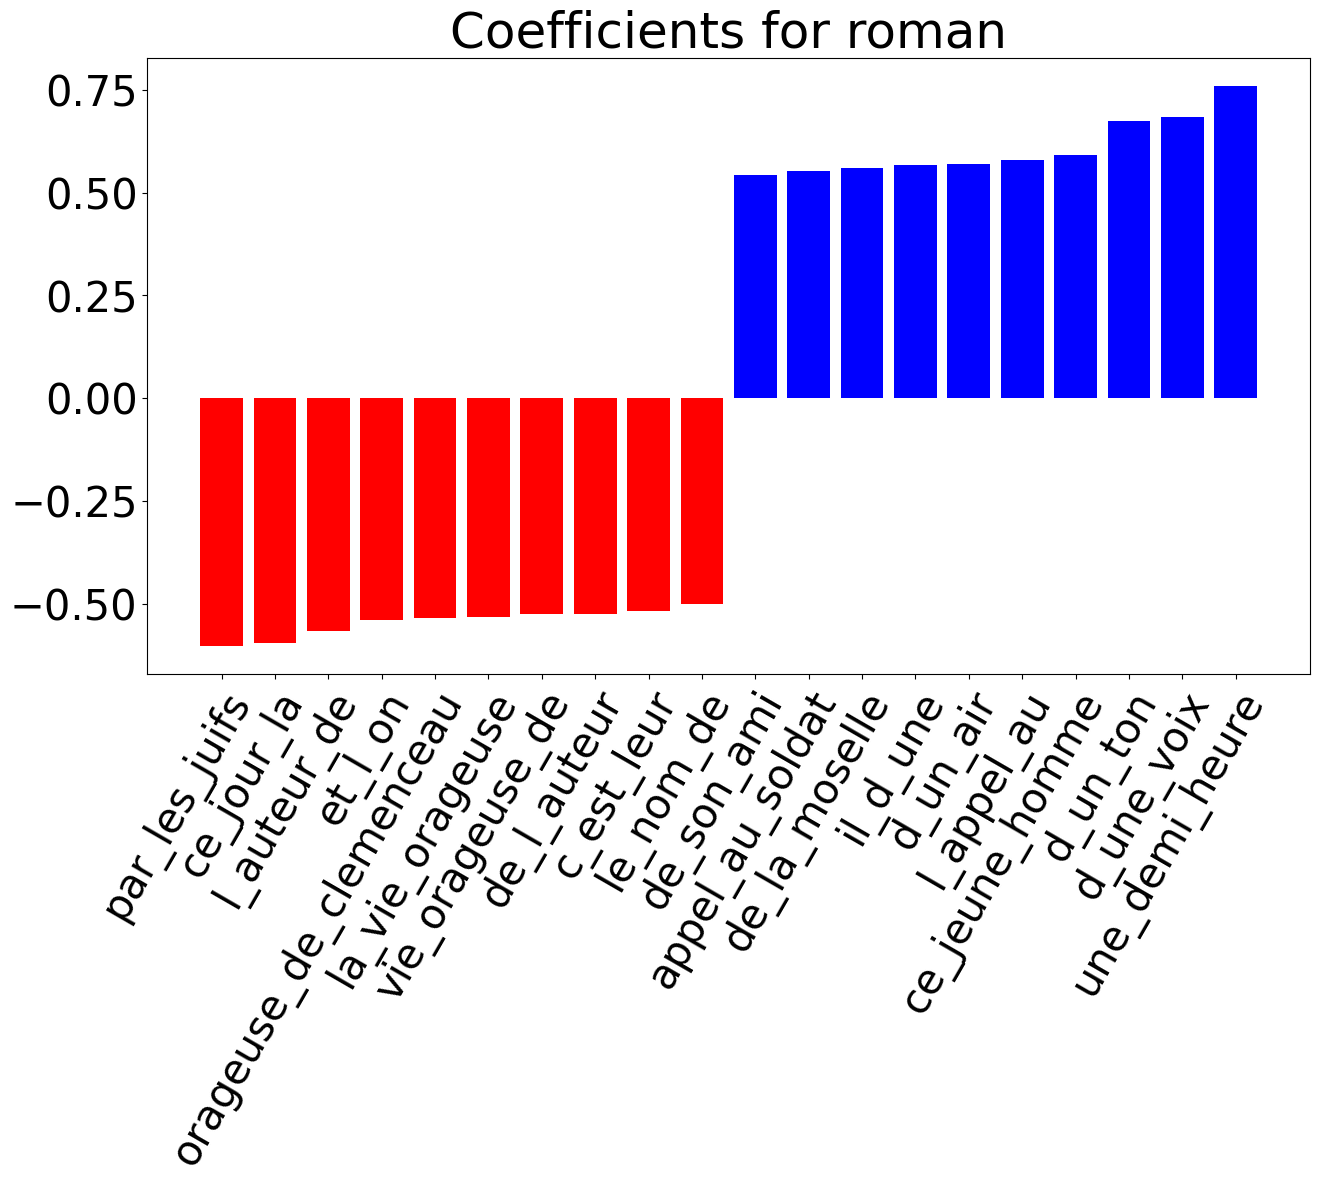
\includegraphics[width=0.70\textwidth]{img/coefs-corpus2-roman.png}
\caption{\textit{Diagramme à barres des coefficients de la classe roman du corpus 2}}
\label{'fig:coefs-corpus2-roman'}
\end{figure}

\begin{figure}[H]
\centering %
\includegraphics[width=0.70\textwidth]{img/coefs-corpus2-mémoire et bio..png}
\caption{\textit{Diagramme à barres des coefficients de la classe mémoire et biographie du corpus 2}}
\label{'fig:coefs-corpus2-mémoire et bio.'}
\end{figure}

\begin{figure}[H]
\centering %
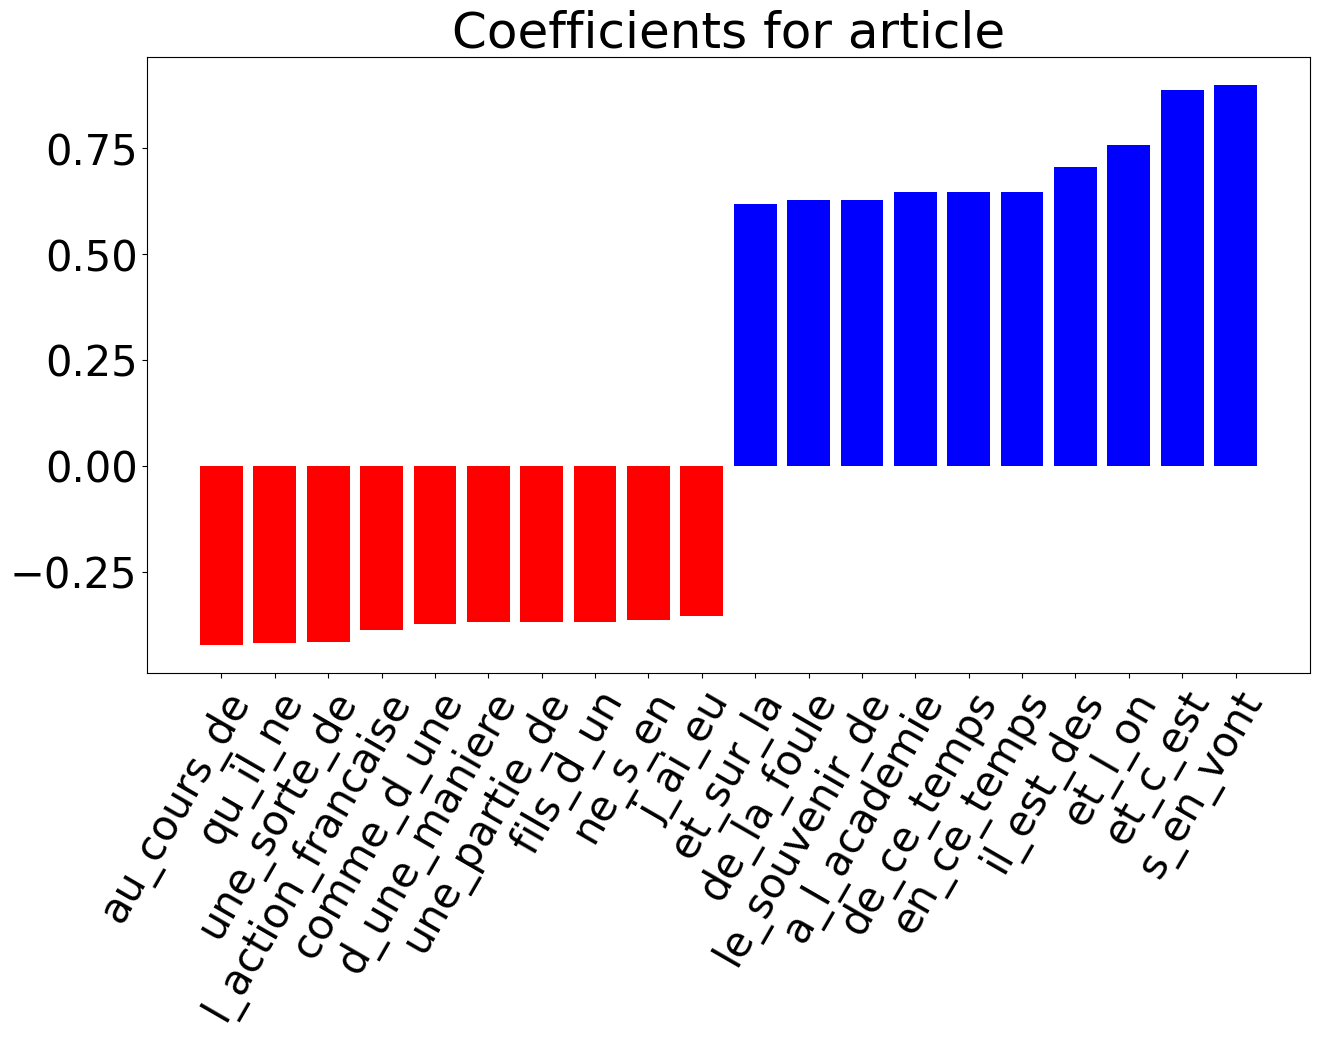
\includegraphics[width=0.70\textwidth]{img/coefs-corpus2-article.png}
\caption{\textit{Diagramme à barres des coefficients de la classe article du corpus 2}}
\label{'fig:coefs-corpus2-article'}
\end{figure}

\begin{figure}[H]
\centering %
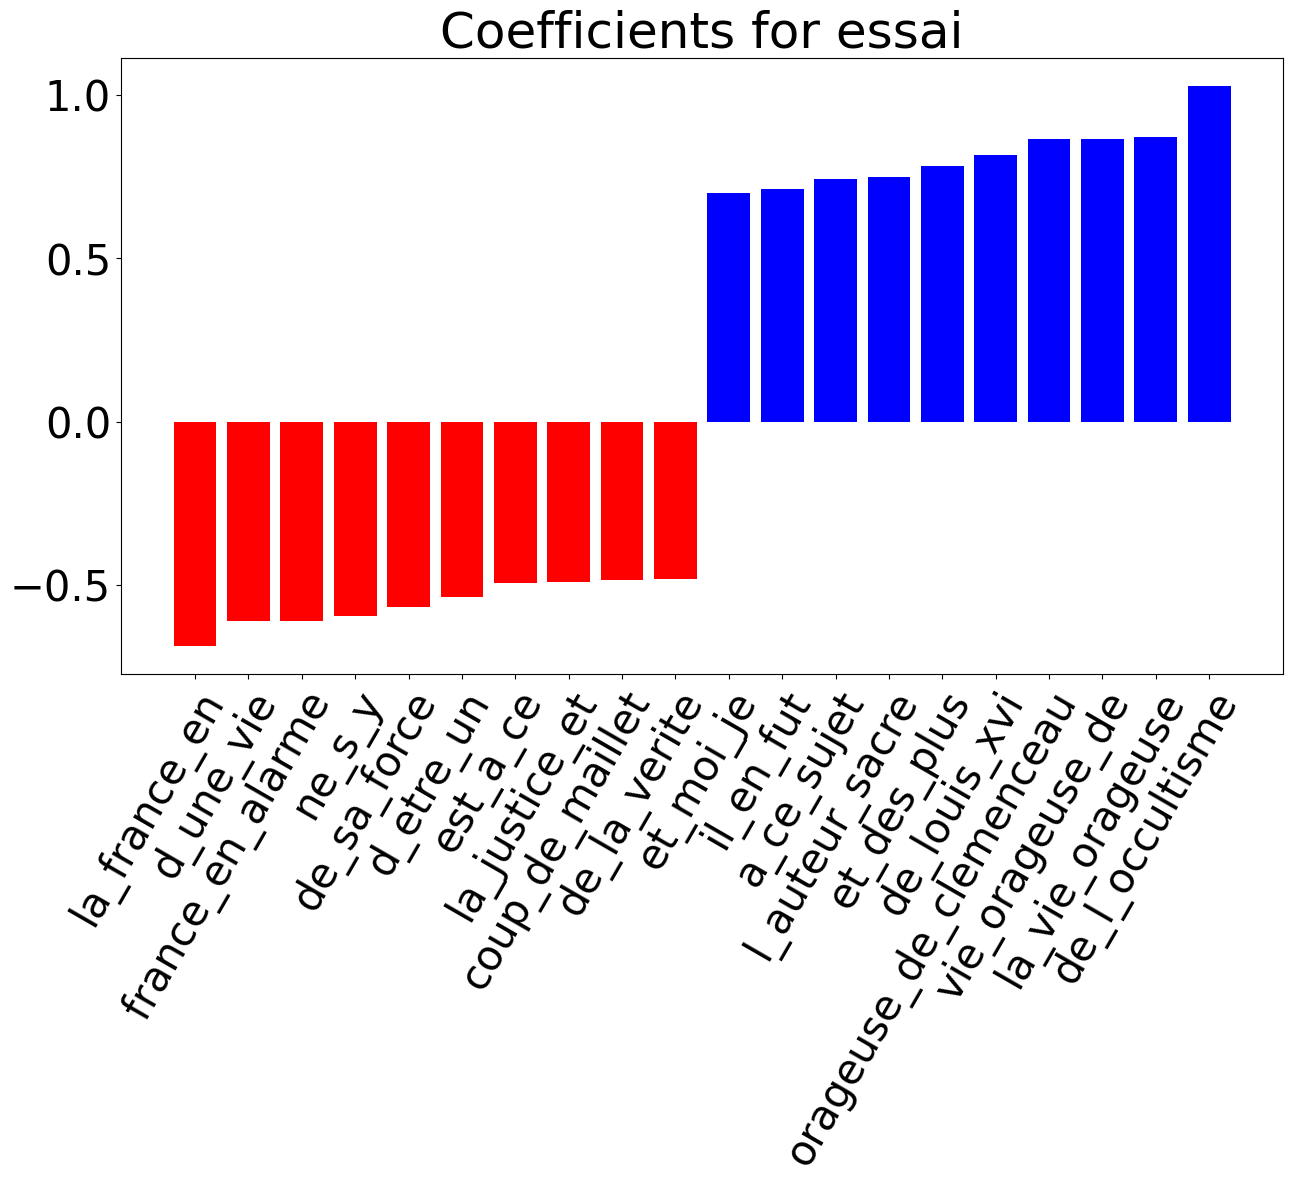
\includegraphics[width=0.70\textwidth]{img/coefs-corpus2-essai.png}
\caption{\textit{Diagramme à barres des coefficients de la classe essai du corpus 2}}
\label{'fig:coefs-corpus2-essai'}
\end{figure}

\begin{figure}[H]
\centering %
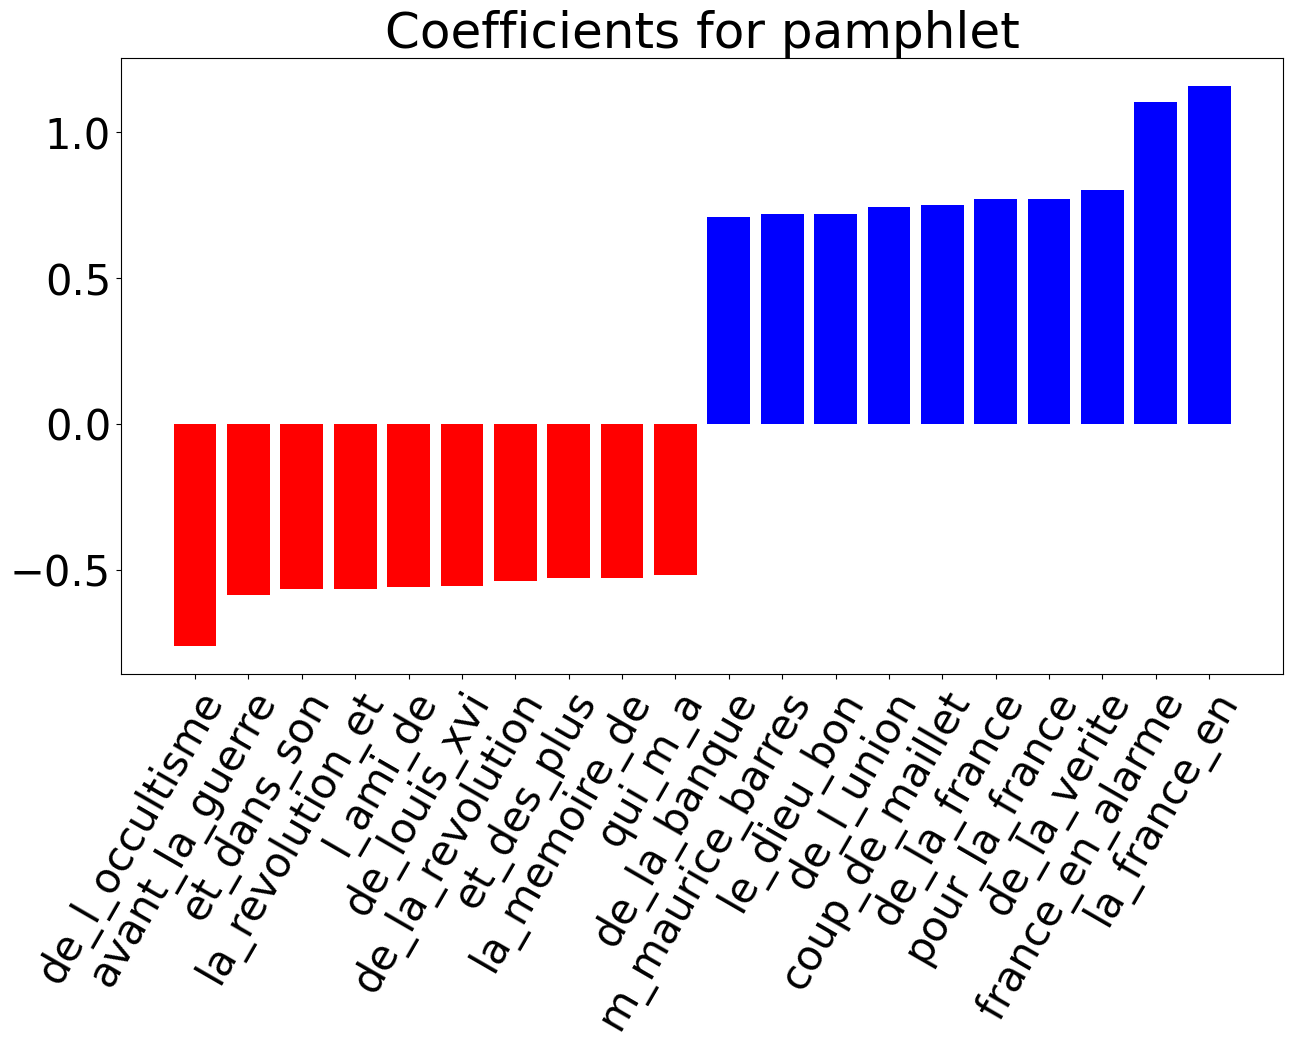
\includegraphics[width=0.70\textwidth]{img/coefs-corpus2-pamphlet.png}
\caption{\textit{Diagramme à barres des coefficients de la classe pamphlet du corpus 2}}
\label{'fig:coefs-corpus2-pamphlet'}
\end{figure}

Pour ce qui est de l'analyse des trigrammes reconnus comme pertinent par la SVM, nous nous permettons de remettre les accents là où il n'y a pas de doute sur leur présence, la SVM ne les prends pas en compte. Et nous unissons les trigrammes de mots qui forment une suite logique. Un problème majeur nous apparaît, une part conséquente des trigrammes sont liés aux titres des ouvrages tel que \enquote{\textit{appel au soldat}}, \enquote{\textit{au seuil de l'apocalypse}}, \enquote{\textit{le salut par les juifs}}, \enquote{\textit{le mendiant ingrat}}, \enquote{\textit{la vie orageuse de Clémençeau}}, \enquote{\textit{la france en alarme}} et quelques autres moins sur tel que \enquote{\textit{le scandale de la vérité}}. Cette apparition des titres d'ouvrages dans les trigrammes les plus représentatifs suppose des erreurs dans l'étape de la post-correction des OCR effectués par nous-même pour une part et des erreurs des versions numériques agrégées dans notre corpus pour une autre part. Ayant éludé ces trigrammes problématiques, nous obtenons quelques éléments sensés pour la classe roman  comme des éléments descriptifs \enquote{\textit{d'un air}}, \enquote{\textit{d'un ton}} et \enquote{\textit{d'une voix}} ainsi que deux trigrammes associés aux personnages \enquote{\textit{de son ami}} et \enquote{\textit{ce jeune homme}}. La classe mémoire mis à part le trigramme \enquote{\textit{de mes livres}} et la classe essai mis à part \enquote{\textit{et moi je}} ne sont pas parlants. La classe article met en lumière plusieurs occurrences de a conjonction \enquote{\textit{et}}. Enfin la classe pamphlet est composé de trigramme plus thématique tel que \enquote{\textit{de la france}} et \enquote{\textit{pour la france}}, \enquote{\textit{le dieu bon}} et \enquote{\textit{coup de maillet}}. On voit un certain lien avec la classe pamphlet du premier corpus ou un lexique du patriotisme frnaçais et de la religiosité poignent légèrement.
L'extraction de ces trigrammes par la SVM montre pour nous un intérêt analytique plus faible du fait de la présence de nom d'ouvrage en leur sein.
Enfin la \textit{table \ref{'tab:matriceconfusioncorpus2'}} montre que les classes de l'essai et du pamphlet sont assez perméables l'une de l'autre. Ces erreurs de prédiction peuvent montrer une plus proche proximité entre ces deux classes. Les erreurs de prédiction des classes vers la classe roman est assez homogène, c'est plus probablement le signal autorial qui doit causer ces erreurs.

\section{Conclusion}

Cette recherche de classification des genres permet de montrer que les textes pamphlétaires sont distinguables des genres narratifs du roman, de la nouvelle et des mémoire et biographie. Néanmoins, pour ce qui est de la distinction entre les articles et les essais vis-à-vis du pamphlet les dissimilitudes sont moins marquées. Cela tient de la proximité formelle des ces groupes. À titre d'ouverture et d'approfondissement, nous aurions aimé déployer les mêmes méthodes avec une approche de stylométrie roulante pour identifier plus clairement, depuis la classe pamphlet, les échantillons qui seraient identifiés comme similaire à l'essai, à l'article ou à la narration, ce qui permettrait d'approfondir les spécificités du pamphlet dans les échantillons de pamphlets dissimilaires de ces trois classes. 
Après avoir appliqué un outil d'analyse supervisé où la SVM recherche ce qui est commun à nos classes comme trait pertinent, nous souhaitons maintenant effectuer une analyse non-supervisé des deux mêmes corpus pour comprendre ce qui automatiquement rapprochent nos textes.

\chapter{Approche non-supervisé}

\section{La recherche de similarité générique non-supervisée}

L'analyse non-supervisé des données textuelles est un large pan de la textométrie et de la stylométrie. Le gain qu'apporte cette approche dans notre méthodologie est de caractériser les rapprochements et similitudes de nos textes sans présupposés sur leur appartenance à une classe. Depuis une même représentation vectorielle de nos corpus, nous cherchons à observer les rapprochements automatiques de nos textes par similitudes. La majorité de ces approches assurent des regroupements par auteurs, le signal autorial dans des genres issus de même champs génériques sont souvent plus fort que le style collectif d'un genre. Néanmoins nous souhaitons observer ce qui automatiquement rapproche nos textes et jouer sur différents paramètres pour au maximum faire émerger le style collectif du pamphlet. Pour nous prémunir d'un biais de comparaison du pamphlet d'un groupe d'auteurs restreint (13 pamphlétaires) face à une grande diversité d'écrivains d'autre genre (le corpus ANR Chapitres, Corpus 1), nous effectuerons une même analyse non-supervisé sur l'ensemble des textes de nos écrivains pamphlétaires (Corpus 2). 
Nous produirons deux chaînes de traitement distinctes, une classification ascendante hiérarchique et une analyse en composantes principales depuis une représentation matricielle de nos corpus ou (\textit{bag-of-words}). 
\par
Le concept de \textit{Bag-of-words}, ou sac de mots permet d'obtenir une représentation vectorielle de nos données textuelles. C'est une représentation simplifiée d'un document texte où l'ordre des mots est ignoré et seule la fréquence d'apparition des mots est prise en compte. Dans cette représentation chaque dimension est un mot unique et la valeur de celle-ci est sa fréquence dans un document donné. Nous parlons de mots, mais cela est vrai pour l'ensemble des \textit{features} que nous pourrions souhaiter extraire depuis les n-grams de caractères jusqu'à des n-grams de mots et bien d'autres encore. Cette seconde approche pour analyser nos données textuelles reprend les bases de l'extraction de \textit{features} de Superstyl que nous implémentons cette fois-ci nous même dans un soucis de contrôle fin des paramètres qui ajustent cette extraction. Notre implémentation permet de choisir le type de \textit{features} à extraire, mots, lemmes ou parti de discours ainsi que le nombre de n-grams ou la fenêtre de \textit{features} à sélectionner comme (1,3) ou (3,3). Les n-grams de (1,3) permettent de constituer une liste de l'ensemble des suites de gram (ou \textit{features}) de longueur 1 jusqu'à 3 par exemple.
La chaîne de traitement que nous mettons en place applique un calcul de fréquence, une normalisation L2 et une standardisation de nos \textit{features} pour obtenir notre représentation vectorielle.
Nous appliquons un calcul de fréquence brute à l'échelle des documents, un processus de normalisation correspondant à une mise à l'échelle des vecteurs de données pour qu'ils aient une certaine propriété, comme une longueur unitaire. Dans ce contexte, la normalisation L2 est utilisée, ce qui signifie que les vecteurs sont ajustés de manière à avoir une longueur euclidienne de 1. La mise à l'échelle standard implique de mettre à l'échelle les données de manière à ce qu'elles aient une moyenne nulle et un écart-type unitaire. Cependant, dans notre traitement, la mise à l'échelle standard est effectuée sans centrer les données autour de zéro car nous avons de nombreuses données creuses.


\section{Méthode choisie}

Nous appliquerons sur chacun des deux corpus définis précédemment pour la SVM notre propre chaîne de traitement. Nous n'effectuons pas d'échantillonnements par soucis de lisibilité des visualisations. Un échantillonement à rendrait le nombre de document à visualiser hors-norme. Nous appliquons un traitement unigram de mots non lemmatisé. Nous avons tenté avec des bigrammes et trigrammes de mots les mêmes analyses, le résultat ne différait peu. D manière itérative nous supprimons les \textit{features} en fonction d'un seuil où les \textit{features} non nulle doivent en être supérieurs. Cette étape de sélection de \textit{features} permet de réduire les variables aberrantes tel que les erreurs d'OCR ou autres \textit{hapax} que nous avons rencontrés au chapitre précédent sur le second corpus mais aussi cela permet de focaliser notre attention sur les valeurs mieux distribuées et potentiellement plus représentative de fait stylistique partagé. Le choix du seuil dépend des données et permet un aller-retour itératifs entre le seuil et les visualisations.
\par
Nous analyserons le fruit de cette matrice de sac de mots par un clustering ascendant hiérarchique et une analyse des Composantes Principales. Par soucis de visibilité nous produisons notre analyse sur des paires de 

\subsection{Clustering Ascendant Hiérarchique}

Le Clustering Ascendant Hiérarchique, abrégé en CAH, appartient à la catégorie des méthodes non supervisées, ce qui signifie qu'il est utilisé pour explorer et regrouper des données sans l'aide de variables cibles prédéfinies comme c'était le cas pour la SVM. Le CAH est particulièrement précieux lorsque l'on cherche à découvrir des structures intrinsèques, des similitudes et des dissimilarités au sein de données complexes et multidimensionnelles, c'est le cas pour nos données textuelles.
Le principe fondamental du CAH est de créer une hiérarchie de regroupements progressivement plus larges en fusionnant itérativement des éléments individuels ou des groupes de données similaires. À chaque étape, le CAH mesure la proximité ou la distance entre les données et combine les éléments les plus proches les uns des autres pour former des groupes de plus en plus vastes. Ce processus de fusion continue jusqu'à ce que toutes les données soient regroupées en un seul ensemble ou selon un critère prédéfini.
La première étape de la fonction implique le calcul de la distance entre les vecteurs représentant les documents dans l'espace des termes. Il existe plusieurs métriques pour définir la distance entre des données textuelles, nous choisissons la distance cosinus. Cette mesure de distance est choisie pour évaluer la similitude entre les documents en prenant en compte les angles entre leurs vecteurs, plutôt que les distances euclidiennes. La matrice de distance ainsi obtenue capture les dissimilarités entre les documents, où des valeurs plus élevées indiquent une dissimilitude plus importante.
À l'aide de la matrice de distance, l'algorithme d'agrégation hiérarchique avec méthode de Ward est employé pour former des groupes de documents en fonction de leurs similitudes. Cette approche construit progressivement une structure de regroupement en fusionnant les groupes les plus proches, en minimisant la variance intra-groupe. Nous générons ensuite une visualisation sous forme de dendrogramme, un diagramme arborescent utilisé pour représenter les regroupements hiérarchiques. Chaque feuille du dendrogramme correspond à un document du corpus. La coloration des branches du dendrogramme est déterminée par le seuil de couleur spécifié. Cette visualisation contrairement à d'autres permet de voir l'ensemble des différentes hiérarchies de cluster.

\subsection{Analyse en Composantes principales}

L'Analyse en Composantes Principales (ACP) est une technique de réduction de la dimensionnalité qui est couramment utilisée en statistiques et en apprentissage automatique pour explorer et analyser des données multidimensionnelles. Son objectif principal est de réduire la complexité d'un ensemble de données en projetant ces données dans un nouvel espace de plus petite dimension tout en conservant autant d'informations que possible. En d'autres termes, elle permet de trouver les combinaisons linéaires des variables d'origine (dans ce cas, les mots dans une matrice Bag-of-Words) qui expliquent le maximum de variabilité dans les données. Cette méthode consiste donc à transformer des variables corrélées en nouvelles variables dé-corrélées entre elles, ce qui est appelé les composantes principales.\par
L'ACP tire son origine du mathématicien Karl Pearson qui la développa au début du XX\ieme siècle. Ce sont ses travaux sur la régression qui le même à traiter des corrélations entre variables non pas pour expliquer une variable à partir des autres mais pour résumer et expliquer l'information contenue dans celles-ci. La formalisation des analyses factorielles dont l'ACP fait partie est déployé par Harold Hotelling, d'ailleurs le terme de transformation de Hotelling est utilisable pour parler de l'ACP. 
Cette capacité à réduire le nombre de dimension et à expliquer une matrice multivariée comme avec notre matrice de fréquences de \textit{features} de un gramme de mot est un atout pour l'explicabilité d'une classification des données.


\section{Résultats et analyses}

\subsection{Sortie du Corpus 1}

Nous présentons donc 3 paires de visualisations associées aux couples pamphlet-roman, pamphlet-mémoire et bio. et pamphlet-nouvelle. Les visualisation en dendrogramme sont accompagnées de trois niveau de légende correspondant à la qualification des textes en genre, auteur et titre, ce choix bien qu'alourdissant la visualisation apporte une meilleure visibilité. Le seuillage pour la colorisation des différentes branches du dendrogramme est fixé arbitrairement. 
La visualisation de l'ACP est fait en graphique bidimensionnel dont nous avons agrémenté la représentation des textes par des couleurs distinguant les genres et les motifs des points pour distinguer les auteurs. Nous omettons la légende des auteurs étant donné que le nom des textes suffit aisément à retrouver ceux-ci, l'intérêt de pouvoir rapidement évaluer l'appartenance d'un texte à un auteur par le choix des motifs de points permet de voir l'agglomération ou non de ceux-ci dans l'espace.

\par
Pour le \textit{dendrogramme \ref{'fig:dendogram-corpus-mix-PamRoman'}} du sous corpus pamphlet roman, nous constatons que la division par genre est fonctionnel sauf pour sept textes pamphlets de Léo Taxil, Laurent Thailade, Jules Vallès et Georges Darien. Nous observons néanmoins que les principaux groupes sont constitués avant tout par le signal autorial. 
Le \textit{graphique de l'ACP \ref{'fig:ACP-corpus-mix-PamRoman'}} quand à lui montre bien deux ensembles que nous soulignons nous même par l'emploi de couleurs distinctes par genre. Les différents motifs de points soulignent la distinction entre auteurs. Nous observons donc des regroupement par auteurs au sein de la division par genre. Le groupe de pamphlet paraît néanmoins très dispersé en opposition avec le groupe de roman. Cette disparité spatiale montre une certaine hétérogénéité des textes pamphlétaires. Nous retrouvons les mêmes cas ambiguës des pamphlets précédents aux plus près du groupe de roman tel que \textit{Les enfants du peuple} de Jules Vallès, \textit{Au pays du Mufle}, \textit{La Noire Idole}, \textit{Les Kalendes et les Ides} et \textit{À travers les Grouins} de Laurent Tailhade, \textit{Les Vrais Sous-Offs} de Darien et la \textit{Lanterne d'un suspendu} de Léo Taxil. Ces textes semblent être soit des cas limites à la frontières de deux genres soit une mauvaise attribution préalable de notre part nous reviendrons sur cela à la fin de cette partie.

\begin{figure}
\centering %
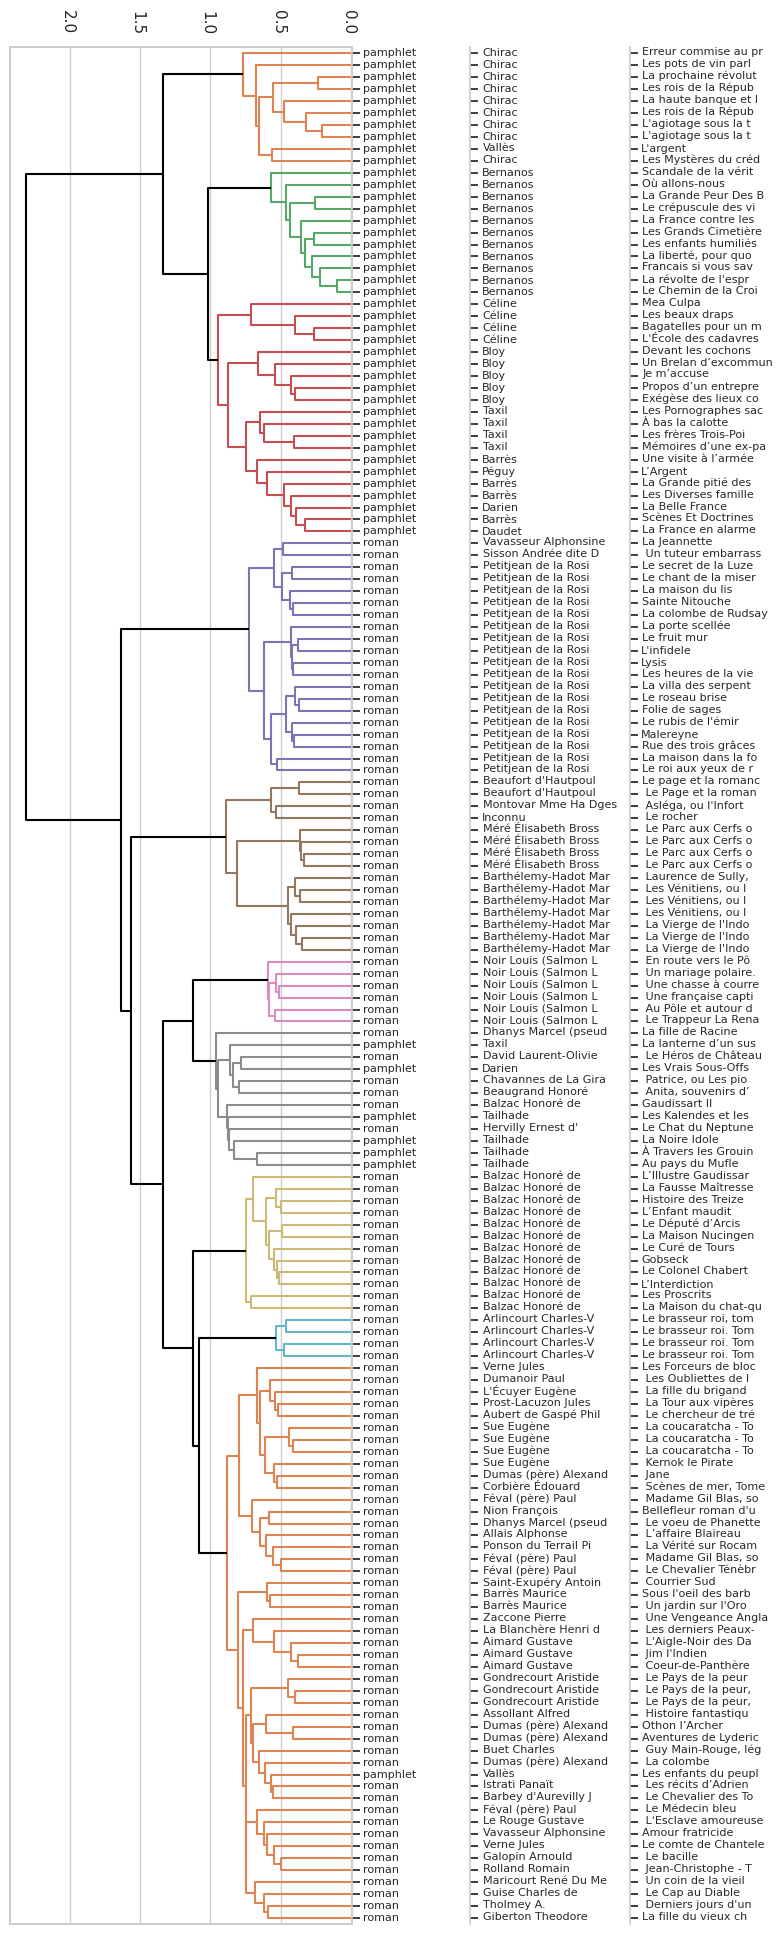
\includegraphics[width=0.60\textwidth]{img/dendogram-corpus-mix-PamRoman.png}
\caption{Dendrogramme de classification ascendante hiérarchique, Corpus 1, Genres pamphlet-roman, 1 n-gram de mot, 7192 / 107397 features, 25 non nulle}
\label{'fig:dendogram-corpus-mix-PamRoman'}
\end{figure}

\begin{figure}[H]
\centering %
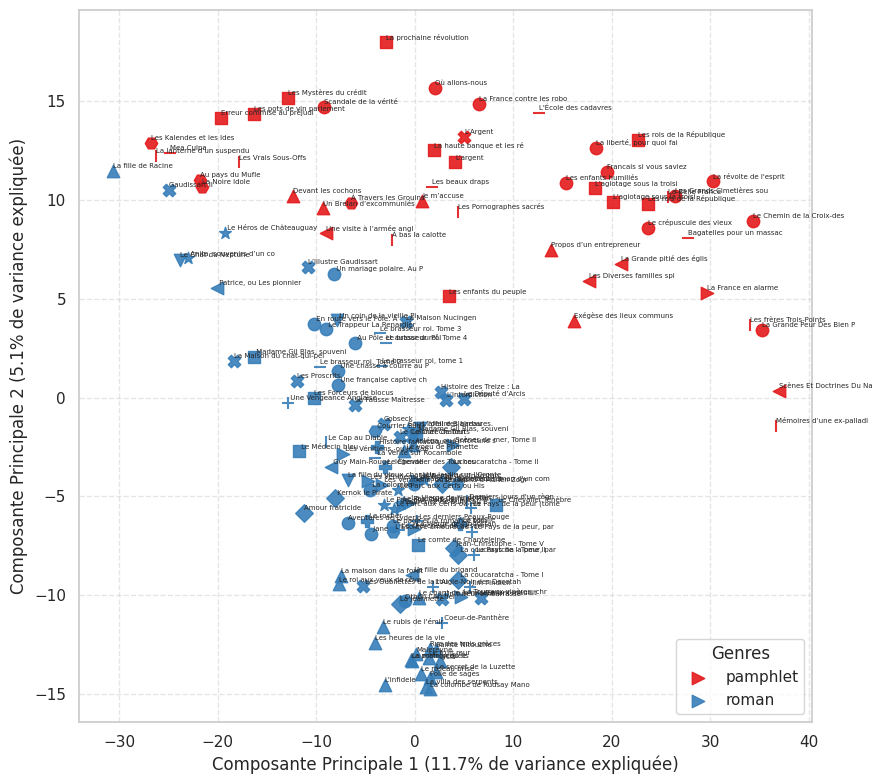
\includegraphics[width=1\textwidth]{img/ACP-corpus-mix-PamRoman.png}
\caption{Analyse en composantes principales, Corpus 1 Genres pamphlet-roman}
\label{'fig:ACP-corpus-mix-PamRoman'}
\end{figure}

Pour le sous corpus formant la paire pamphlet-mémoire et biographie, nous observons exactement les mêmes textes que précédemment être exclue de l'ensemble constitué de pamphlet. Trois mémoires et bio. sont elles-mêmes inclus dans l'ensemble de pamphlet. Les \textit{Lettres de Bayreuth} de Charles Henri Tardieu sont un cas ambigu, la forme même du recueil de lettres avec un style mélangé journalistique et essayistique et le ton très incarné assez proche de la figure des pamphlétaires tend à montrer les limites d'une approche statistique. Voici un bref extrait assez représentatif de ce ton :\\

\par\textit{ Bayreuth, 14 août 1876, matin 
 Vous me demandez la vérité vraie, c'est fort bien, mais la mienne, ma vérité à moi, ne sera peut-être pas vraie pour vous, et la vôtre pourrait bien être la fausseté même pour les quinze cents personnes qui ont acclamé hier soir l'auteur de l'Anneau du Nibelung. Il y a vingt vérités vraies, il y en a cent, il y en a mille en art, comme en religion et en politique. Je renonce à chercher la plus vraie de toutes, la seule vraie, la vérité des vérités. Tout ce que vous pouvez exiger de votre correspondant, c'est la sincérité. Permettez donc que je vous donne franchement et tout bêtement mon sentiment.} Lettres de Bayreuth, Charles Henri Tardieu.

Cela se rapproche de ce qu'à pu écrire Léon Bloy dans ses chroniques du Chat Noir rassemblé dans \textit{Propos d'un entrepreneur de démolitions} Ce texte issu de l'ARN Chapitres est donc un cas limite en soi. Le second et troisième cas spéciaux sont les deux tomes du \textit{Voyage d'un jeune grec} d'Hippolyte Mazier du Heaume. Ce texte semble aussi être un cas limite, le thème est artistique mais le ton est virulent.
La visualisation de l'ACP montre une grande dispersion des pamphlets face à une certaine homogénéité du groupe de mémoire, excepté une porosité entre les cas limite de pamphlet comme précédemment, les cas de mémoires et biographies spécieux auquel nous pouvons ajouter \textit{Aden Arabie} de Paul Nizan, nous avions évoqués ce texte qui fut dans le cas de la SVM aussi un cas limite que nous retrouvons ici.

\begin{figure}[H]
\centering %
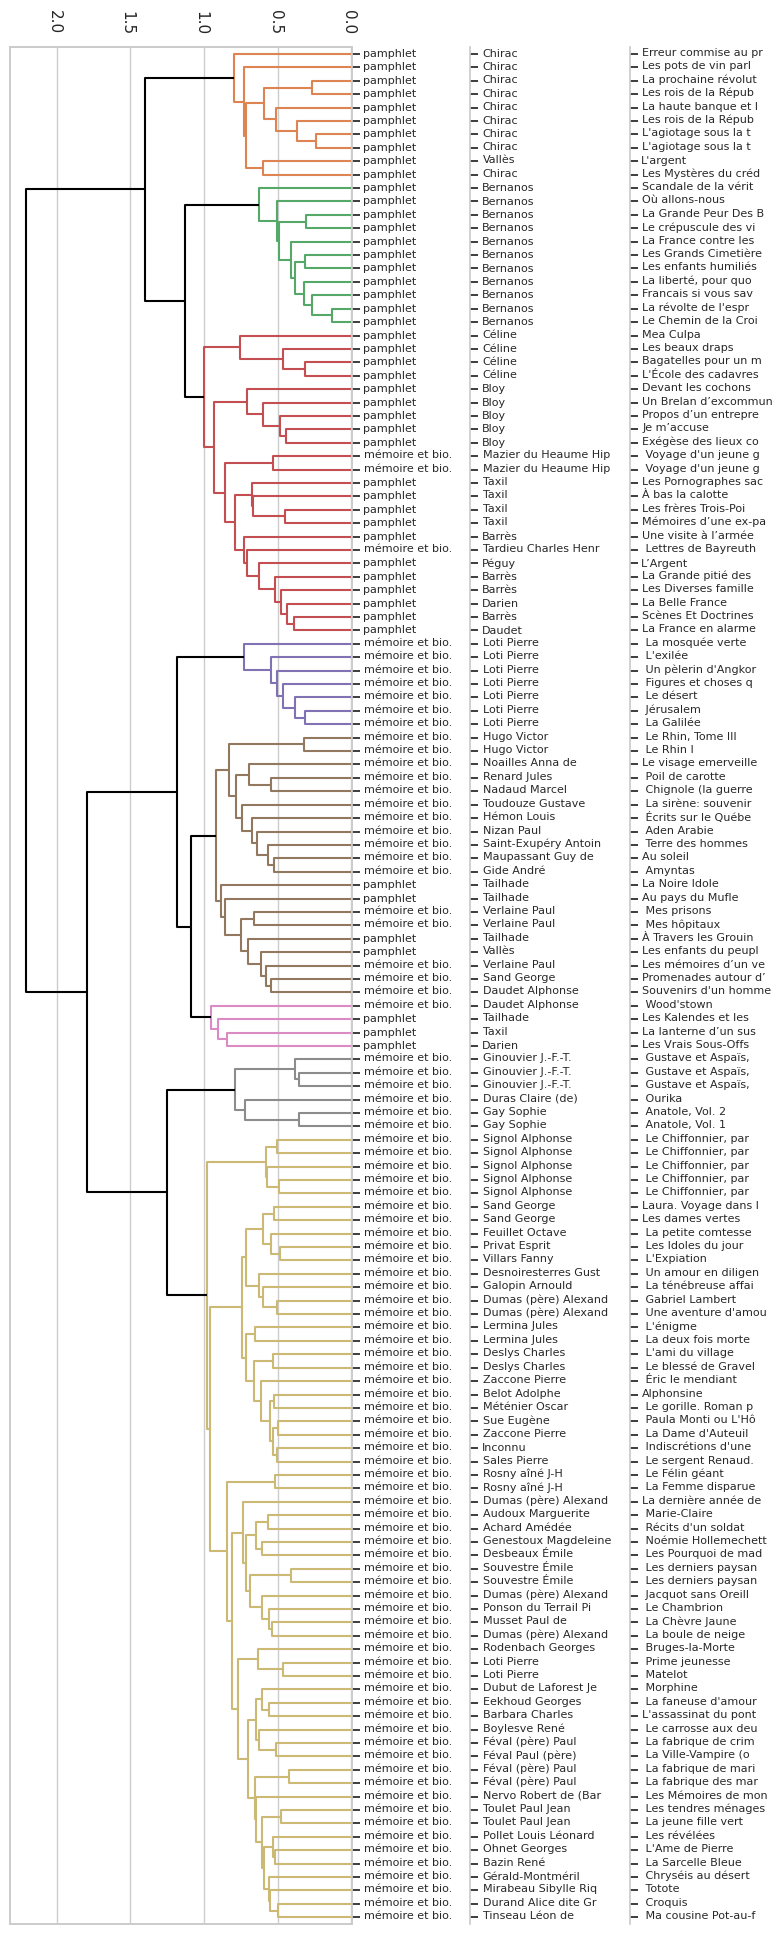
\includegraphics[width=0.60\textwidth]{img/dendogram-corpus-mix-PamMem.png }
\caption{Dendrogramme de classification ascendante hiérarchique, Corpus 1, Genres pamphlet-mémoire et biographie, 1 n-gram de mot, 8833 / 110741 \textit{features}, 25 non nulle}
\label{'fig:dendogram-corpus-mix-PamMem'}
\end{figure}

\begin{figure}[H]
\centering %
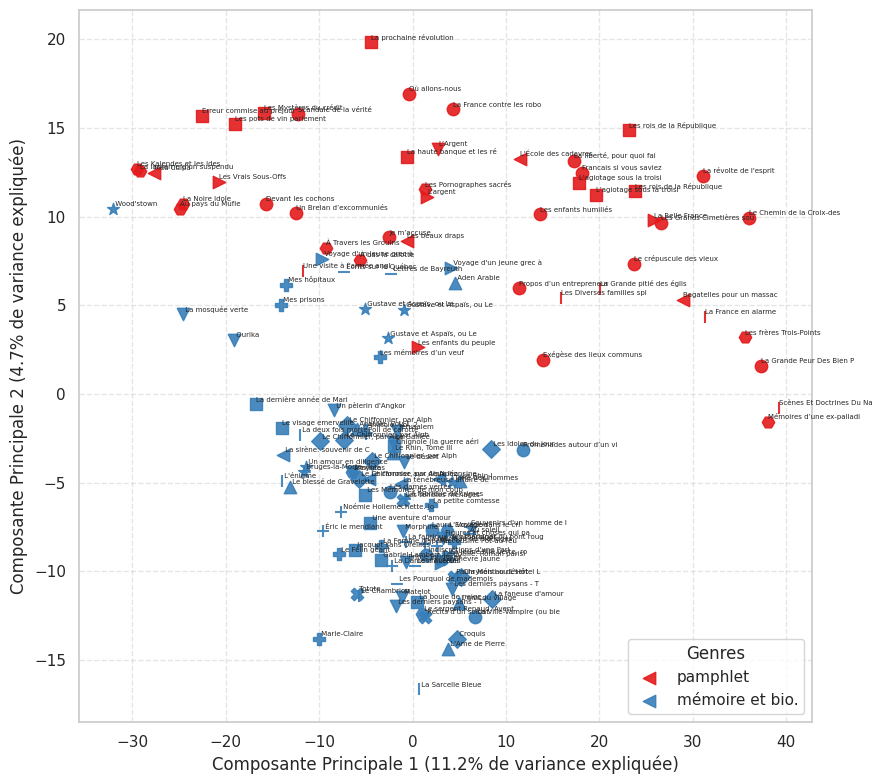
\includegraphics[width=1\textwidth]{img/ACP-corpus-mix-PamMem.png}
\caption{Analyse en composantes principales, Corpus 1, Genres pamphlet-mémoire et biographie}
\label{'fig:ACP-corpus-mix-PamMem'}
\end{figure}


Pour cette troisième paire pamphlet-nouvelle nous constatons que les mêmes textes classés pamphlet par nos soins qui se trouvaient placés hors des branches pamphlétaires pour les dendrogrammes précédent se retrouvent hors de la branche pamphlétaire du \textit{dendrogramme \ref{'fig:dendogram-corpus-mix-PamNouvelle'}} hormis \textit{Les enfants du peuple} de Jules Vallès qui cette fois-ci fait parti de cette branche pamphlétaire, cela permet de remettre en équilibre sa dimension de cas limite. Pour le reste des textes spécieux pamphlets, nous pouvons encore constater leur positionnement spatial comme en marge des deux ensembles.

\begin{figure}[H]
\centering %
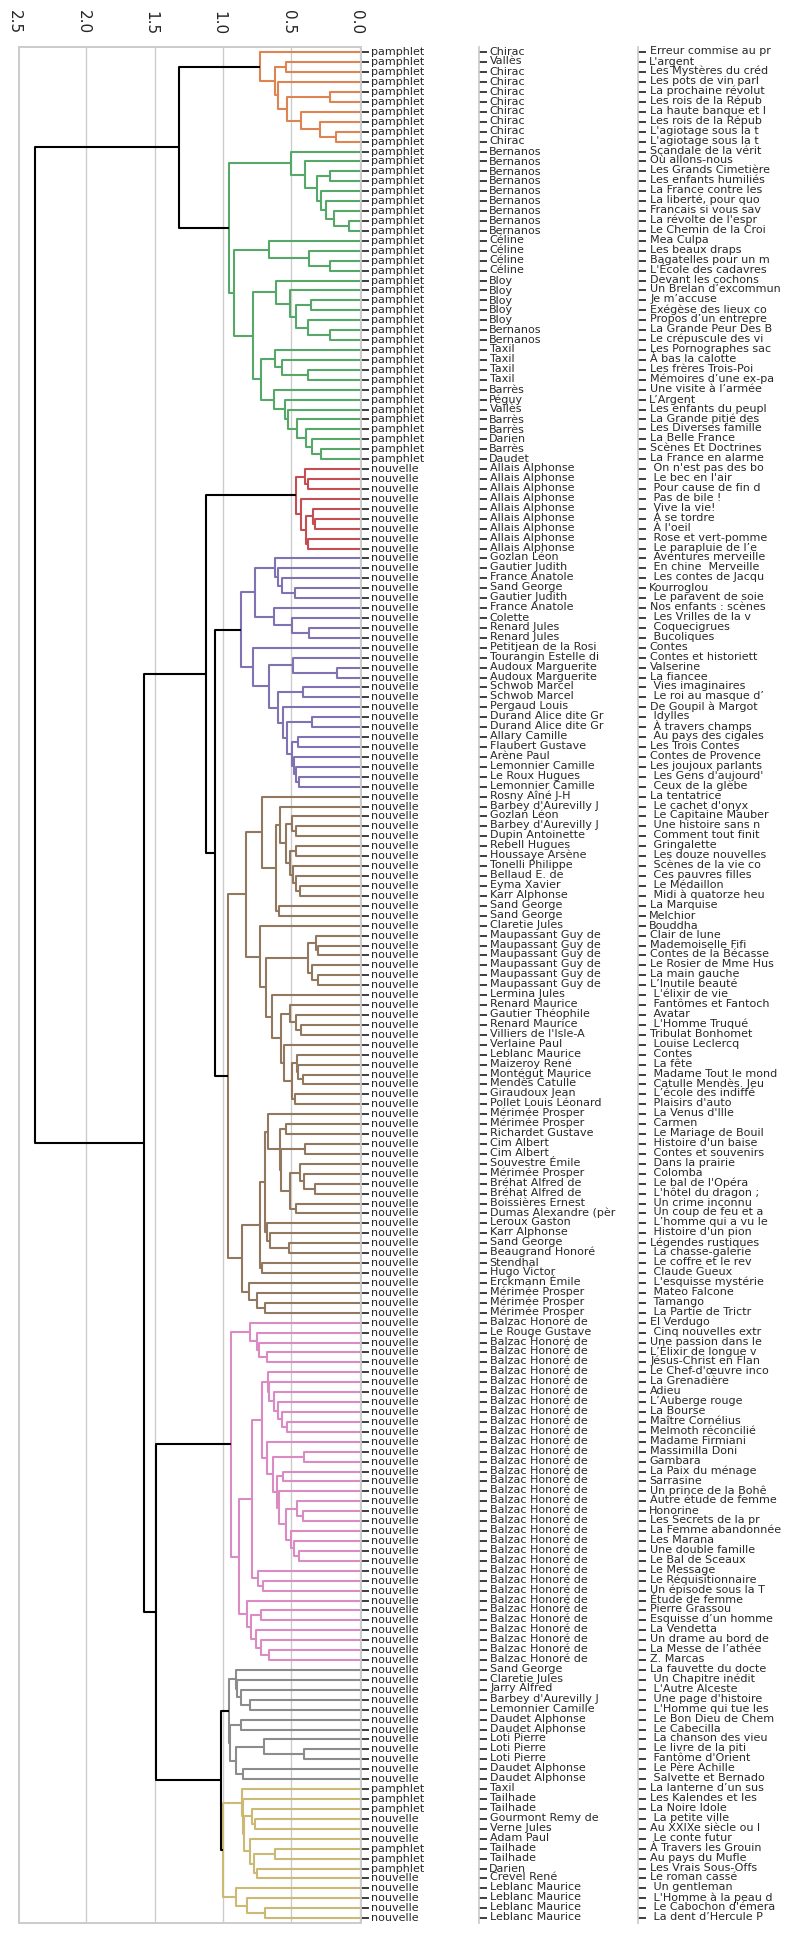
\includegraphics[width=0.60\textwidth]{img/dendogram-corpus-mix-PamNouvelle.png}
\caption{Dendrogramme de classification ascendante hiérarchique, Corpus 1, Genres pamphlet-nouvelle, 1 n-gram de mot, 5700 / 113137 \textit{features}, 40 non nulle}
\label{'fig:dendogram-corpus-mix-PamNouvelle'}
\end{figure}


\begin{figure}[H]
\centering %
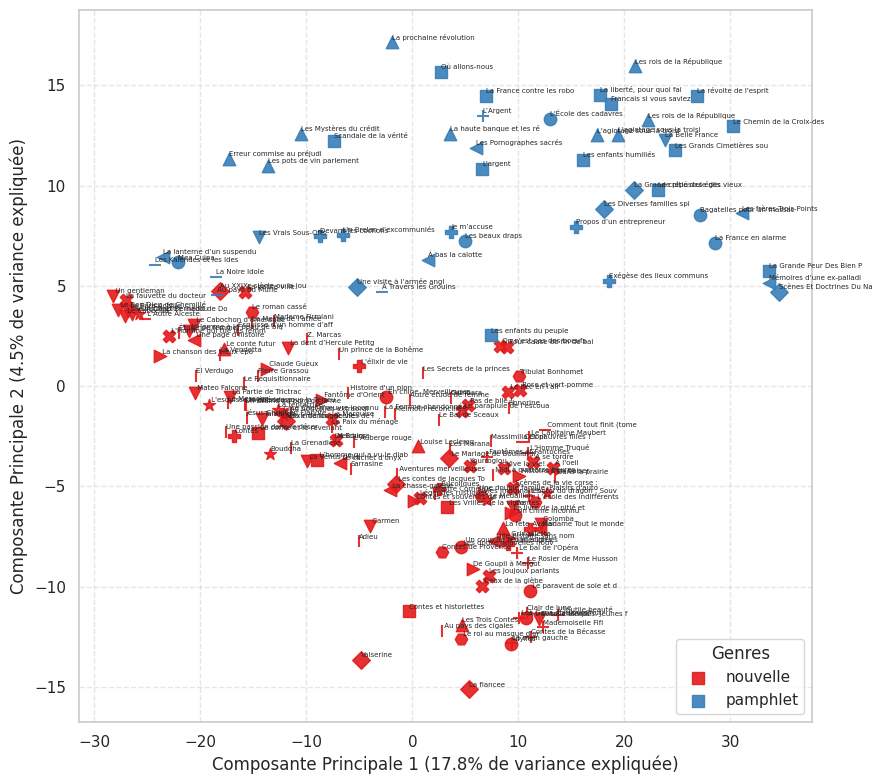
\includegraphics[width=1\textwidth]{img/ACP-corpus-mix-PamNouvelle.png}
\caption{Analyse en composantes principales, Corpus 1 Genres pamphlet-nouvelle}
\label{'fig:ACP-corpus-mix-PamNouvelle'}
\end{figure}

Ces différentes analyses tendent à montrer une nette distinction entre le champ générique de la narration représenté par les mémoires et biographies, les romans, les nouvelles et les pamphlets.
La visualisation de la classification ascendante hiérarchique en dendrogramme nous laisse à penser que cette distinction est franche et que le pamphlet forme un ensemble aussi cohérent que les différents genres mis en comparaison. Néanmoins la visualisation de l'analyse en composantes principales nous montre une dispersion plus grande du groupe de pamphlet qui est bien moins homogène dans sa répartition spatiale que pour les genres d'où nous le comparons.

\subsection{Sortie du Corpus 2}

Nous appliquons donc les mêmes méthodes sur ce second corpus uniquement composés des textes que nous avons agrégés des auteurs pamphlétaires. Cette seconde salve d'analyse à pour but d'observer la force du signal générique face à celle du signal autorial. Étant donné que l'ensemble des textes se divise en une poignée d'auteurs, les similarités des textes risquent fort de se faire par auteurs. Ayant ce biais à l'esprit nous savons que les visualisations en dendrogramme risquent d'être moins pertinentes car plus aptes à montrer un rapprochement par auteurs. Mais nous espérions que la visualisation de l'ACP puisse quand même apporter des regroupements génériques. Nos analyses sur le corpus précédent ont montré une claire frontière entre le champ générique de la narration et celui du pamphlet, ce que nous retrouverons ici malgré le bruitage du signal autorial. Ce qui nous intéresse plus particulièrement sont les comparaisons des pamphlets face aux essais et aux articles. En effet, ces trois genres partagent une proximité générique bien supérieur à ce que partagent, le pamphlet et le roman par exemple. 

\begin{figure}
\centering %
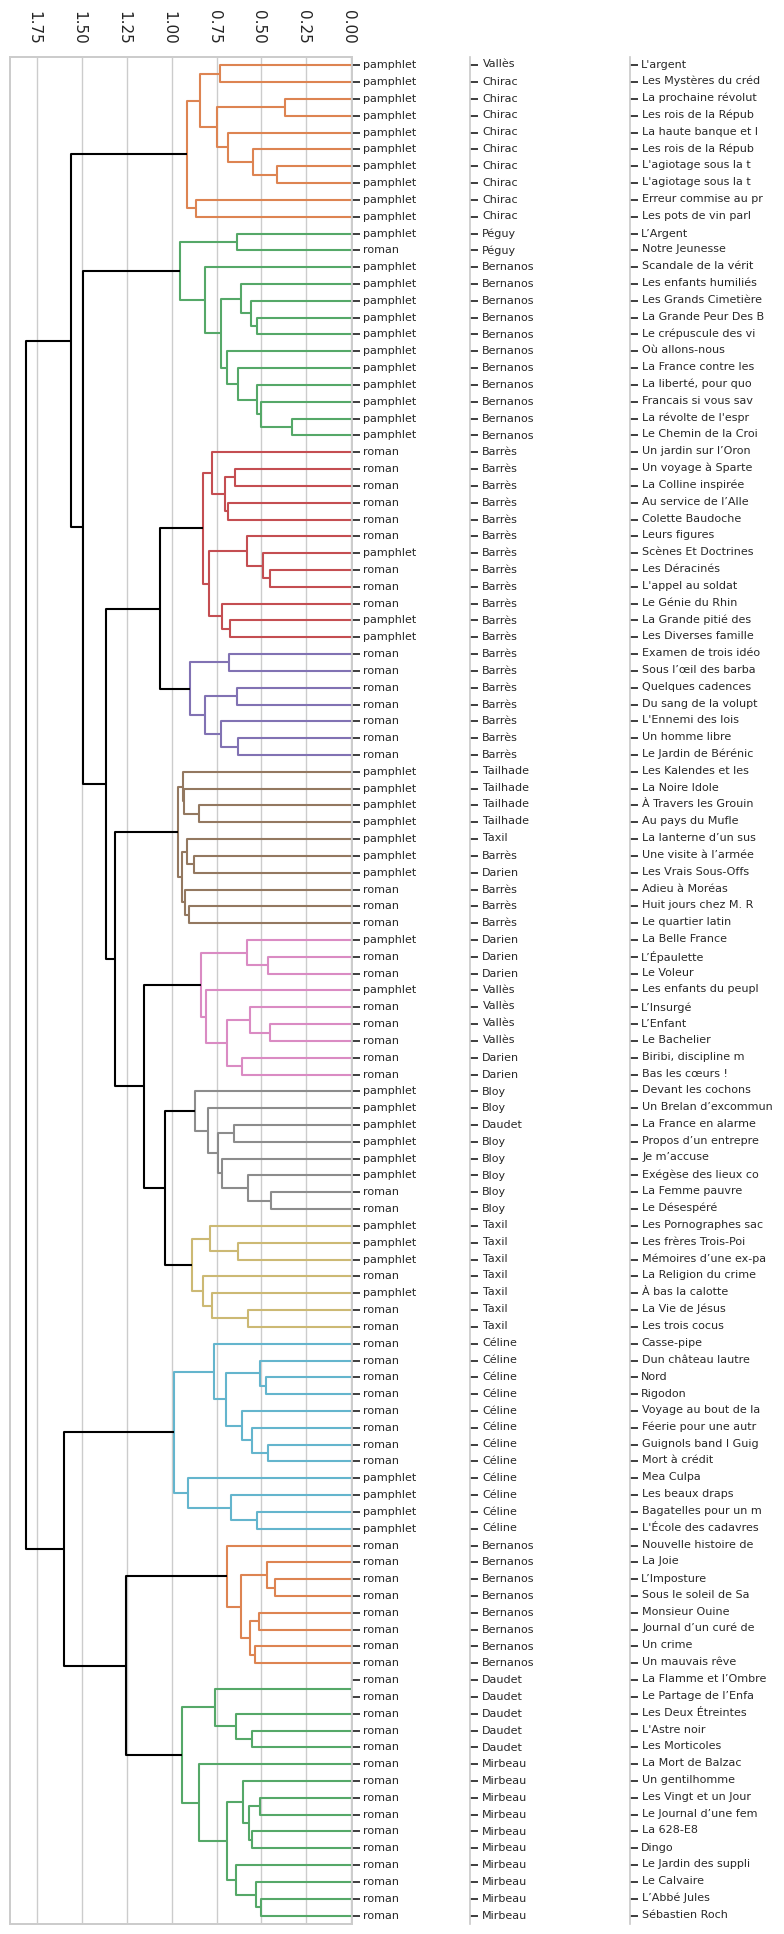
\includegraphics[width=0.6\textwidth]{img/dendogram-corpus-2-PamRoman.png}
\caption{Dendrogramme de classification ascendante hiérarchique, Corpus 2, Genres pamphlet-roman, 1 n-gram de mot, 22272 / 131547 \textit{features}, 25 non nulle}
\label{'fig:dendogram-corpus-2-PamRoman'}
\end{figure}

\begin{figure}[H]
\centering %
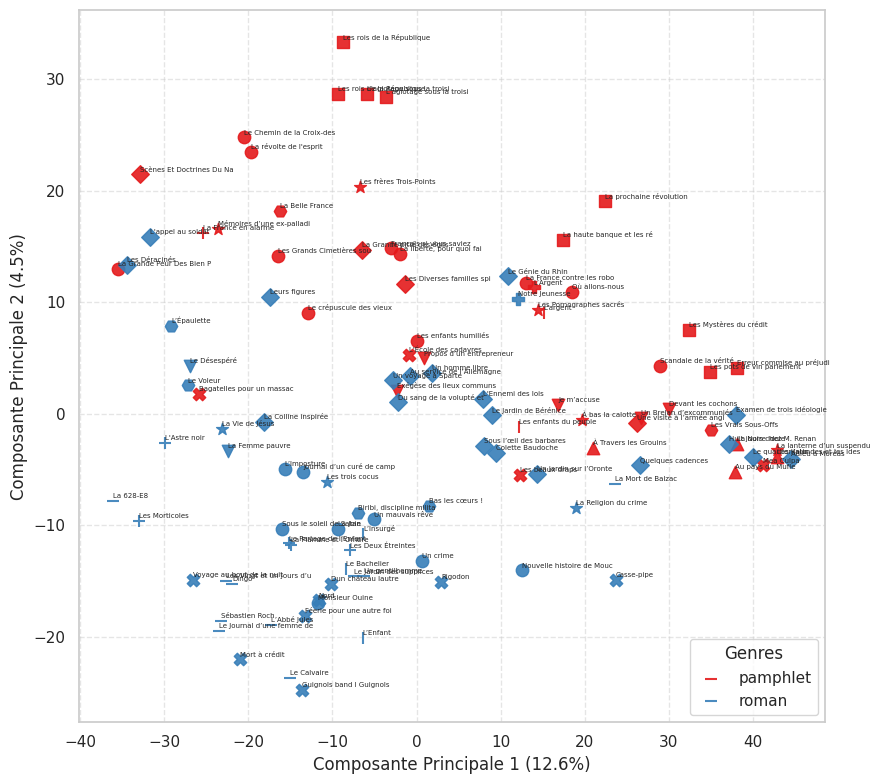
\includegraphics[width=1\textwidth]{img/ACP-corpus-2-PamRoman.png}
\caption{Analyse en composantes principales, Corpus 1 Genres pamphlet-roman}
\label{'fig:ACP-corpus-2-PamRoman'}
\end{figure}

Pour la comparaison du pamphlet et du roman, nous observons une plus grande difficulté à saisir la hiérarchisation des branches de la visualisation en dendrogramme. La formation des branches oscille entre une division par auteur et par genre. Par exemple pour les textes de Georges Bernanos, la division s'effectue par genre assez clairement, alors que pour Louis-Ferdinant Céline, c'est bien l'attribution autoriale qui prédomine. Les choix de la formation des branches suivant le clustering ascendant hiérarchique montre bien une incertitude sur la capacité à classer les textes en genre. L'exemple de la répartition fragmentée des textes de Jules Vallès entre signal autorial et générique renforce cet avis. Nous nous attendions à ce fort bruitage. Les cas de pamphlet spécieux du précédent corpus ne réapparaissent pas avec la même évidence, \textit{Les enfants du peuple} de Jules Vallès est associé au roman de ce même auteur avec une branche divergente là où la majorité des autres cas spécieux se retrouvent dans la même branche au coté de trois romans de Maurice Barrès. Nous pouvons soutenir que ces cas ambigus de pamphlets continuent de l'être dans ce corpus. Cette indisctinction entre classification générique ou autorial rend plus difficile une analyse complète.
Nous retrouvons cette oscillation dans la visualisation de l'analyse en composantes principales, où bien que de grande tendance de groupe émerge entre pamphlet et roman, ces deux ensemble n'ont pas de marges et même partage une union assez marquée. La proximité par auteur bien qu'évidente n'est pas aussi intuitive que nous le présentions. Les exemples de l'emplacement de \textit{Bagatelles pour un massacre} ou de l'ensemble des textes de Maurice Barrès réparti à la jonction des deux ensembles montrent une incapacité à établir clairement une distinction de genre par cette méthode sur ce corpus.

\par
La comparaison des mémoires et biographies face aux pamphlets, ainsi que des nouvelles faces aux pamphlets souffre d'une indigence de diversité d'auteurs. La majorité des mémoires et biographies sont écrites par Léon Bloy ce qui ne permet pas une réelle comparaison de genre, le biais induit est trop grand. Et le nombre de nouvelle est cinq fois moins grand que le nombre de pamphlet. Nous ne nous tardons pas sur ces cas biaisés, néanmoins les visualisations en \textit{dendrogramme \ref{'fig:dendogram-corpus-2-PamMem'}} et celle de \textit{l'ACP \ref{'fig:ACP-corpus-2-PamMem'}} de la comparaison des mémoires et biographies ainsi que le \textit{dendrogramme \ref{'fig:dendogram-corpus-2-PamNouvelle'}} et la visualisation de \textit{l'ACP \ref{'fig:ACP-corpus-2-PamNouvelle'}} sont accessibles depuis l'annexe.

\begin{figure}[H]
\centering %
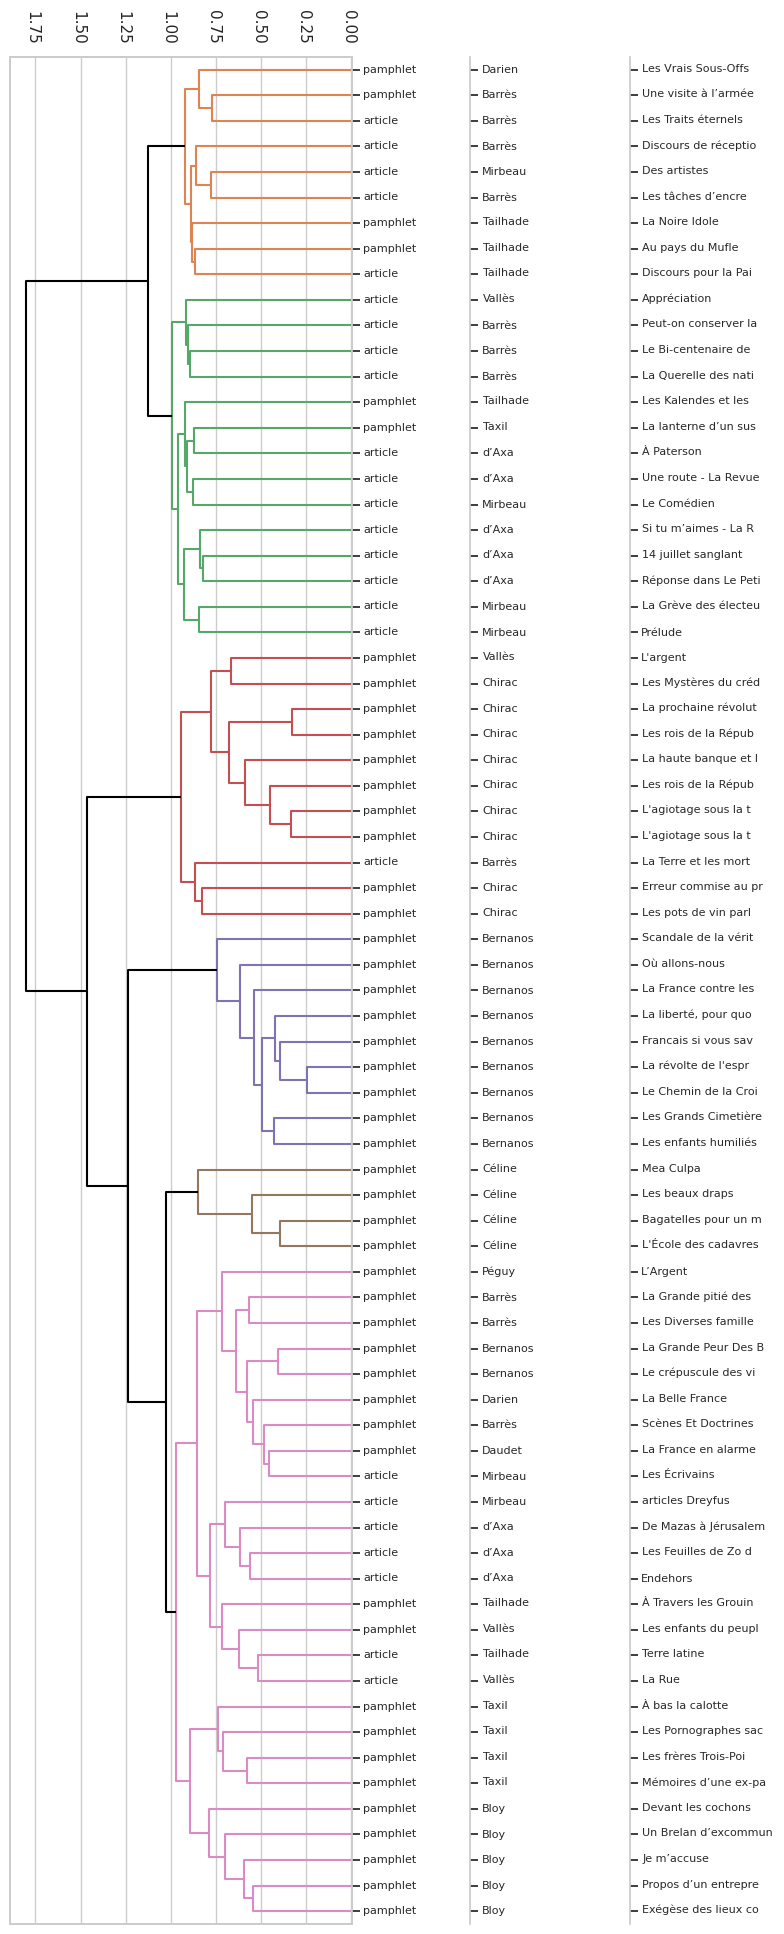
\includegraphics[width=0.60\textwidth]{img/dendogram-corpus-2-PamArticle.png}
\caption{Dendrogramme de classification ascendante hiérarchique, Corpus 2, Genres pamphlet-article, 1 n-gram de mot, 11650 / 92139 \textit{features}, 40 non nulle}
\label{'fig:dendogram-corpus-2-PamArticle'}
\end{figure}


\begin{figure}[H]
\centering %
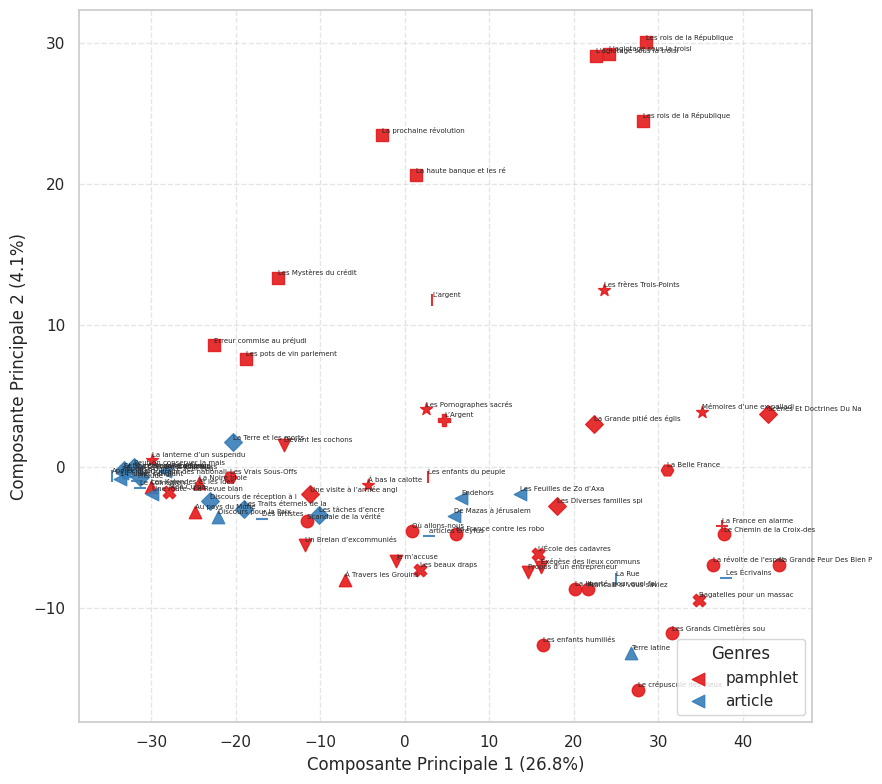
\includegraphics[width=1\textwidth]{img/ACP-corpus-2-PamArticle.png}
\caption{Analyse en composantes principales, Corpus 2 Genres pamphlet-article}
\label{'fig:ACP-corpus-2-PamArticle'}
\end{figure}

La comparaison des pamphlets et des articles rend compte d'une difficulté similaire de visualisation et d'interprétation des résultats. Sur le dendrogramme il semble y avoir des regroupements par genre en deux branches majoritairement pamphlet pour l'une et majoritairement article pour l'autre. Au sein de ces branches le regroupement par auteurs est le plus commun. Néanmoins sur les six textes qualifiés de pamphlet présent dans la branche article, nous retrouvons nos cas de pamphlets spécieux avec \textit{Les Vrais Sous-Offs}, \textit{La Noire Idole}, \textit{Les Kalendes et les Ides} et \textit{La Lanterne d'un suspendu} mais aussi \textit{Au pays du Mufle} qui était un cas ambigu pour la comparaison avec le roman.
Pour les cas des articles regroupés dans des branches contenant majoritairement des pamphlets, nous trouvons deux textes d'Octave Mirbeau, trois de Zo d'Axa, un de Laurent Tailhade et un de Jules Vallès. Il est intrigant de retrouver deux articles d'O. Mirbeau et de Z. d'Axa dans la branche pamphlet alors même qu'il y a des articles de ces mêmes auteurs dans la branche principale des articles. La force du signal autorial devrait à notre sens devoir les regrouper bien plus logiquement. En se tournant vers l'analyse en composantes principales nous constatons que les articles et les pamphlets semblent spatialement peu distinguables. Des regroupement par auteur s'observent dans la plupart des cas. Le groupe de pamphlet est assez dispersé notamment avec les textes d'Auguste Chirac. Nous constatons que les pamphlets spécieux, nos mêmes cas ambigus, sont les plus proches de la zone très agglomérée du groupe des articles. Et que les articles qui étaient regroupés dans la branche pamphlet du dendrogramme sont totalement excentré du groupe d'article de la visualisation de l'ACP. En laissant de coté le cas des pamphlets spécieux, nous pouvons donc affirmer que les unigrammes de mots supposent une proximité entre les pamphlets et les articles des mêmes auteurs de manière plus significatif qu'entre les pamphlets et les romans. À  ce stade nous ne pouvons pas interpréter les raisons de cette proximité avec nos analyses CAH et ACP mais cela se révèle à l'échelle des fréquences de mots.


\begin{figure}[H]
\centering %
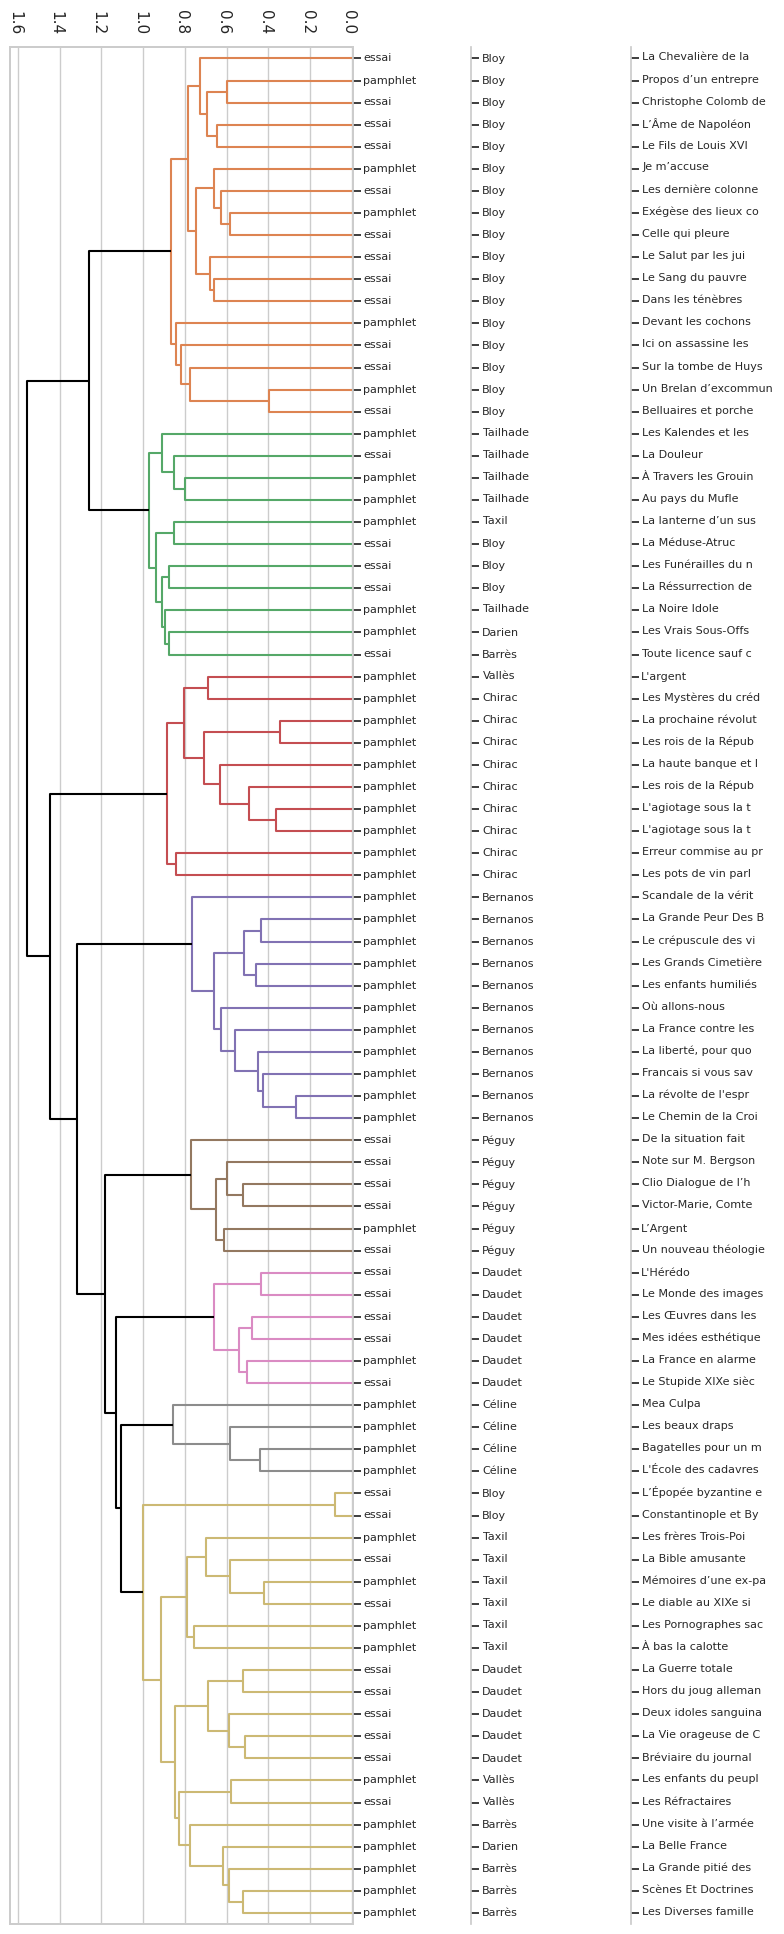
\includegraphics[width=0.60\textwidth]{img/dendogram-corpus-2-PamEssai.png}
\caption{Dendrogramme de classification ascendante hiérarchique, Corpus 2, Genres pamphlet-essai, 1 n-gram de mot, 15492 / 110867 \textit{features}, 40 non nulle}
\label{'fig:dendogram-corpus-2-PamEssai'}
\end{figure}


\begin{figure}[H]
\centering %
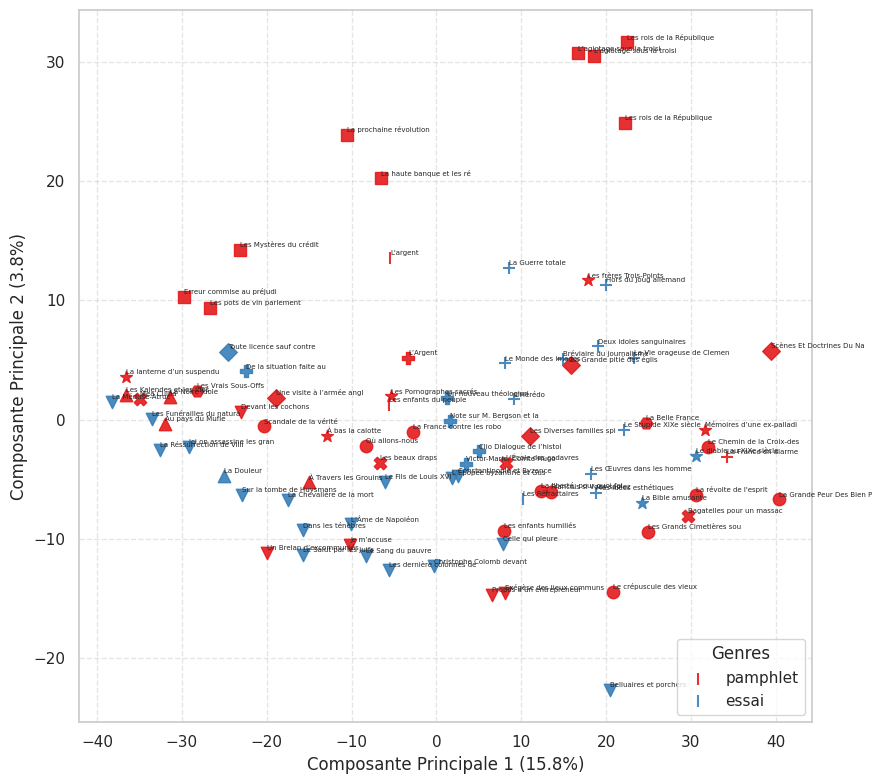
\includegraphics[width=1\textwidth]{img/ACP-corpus-2-PamEssai.png}
\caption{Analyse en composantes principales, Corpus 2 Genres pamphlet-essai}
\label{'fig:ACP-corpus-2-PamEssai'}
\end{figure}

La dernière comparaison entre pamphlet et essai est la plus intéressante pour cette étude. Marc Angenot, comme nous avons pu l'expliquer dans l'introduction, fait du pamphlet et de l'essai une appartenance commune aux discours enthymématique et doxologique. Cette appartenance suppose donc de pouvoir observer des faits de langues communs aux pamphlet et essai. Malgré cette grande proximité nous souhaitons pouvoir observer une divergence entre ces deux ensembles. Lorsque l'on se tourne vers cette dernière visualisation en dendrogramme, nous ne pouvons à première vu observer uniquement une ramification par auteur. Une branche comporte plus de pamphlet mais la distinction est ténu voir quasi nulle. Nos pamphlets spécieux se retrouvent tous dans une branche composée uniquement d'essais d'autres auteurs hormis un essai de Laurent Tailhade. La constance de la répartition de ces pamphlets spécieux souligne une dissemblance forte de ces textes avec le reste de l'ensemble de nos pamphlets. Nous pouvons souligner que certains essais de Léon Bloy, bien qu'une branche identifie la majorité de ces textes pamphlets et essais ensemble, se retrouvent dans des branches très éloignés, nous ne savons pas interpréter cet écart.
La visualisation de l'analyse en composantes principales, \textit{figure \ref{'fig:ACP-corpus-2-PamEssai'}}, ne nous permet pas de déceler une distinction entre le groupe de l'essai et celui du pamphlet, les deux étant indiscernables spatialement. Nous retrouvons encore les textes d'Auguste Chirac assez excentré de l'ensemble. Cette absence de distinction nous force à constater que l'analyse de la fréquence des unigrammes de mots ne sont pas une variable pertinente pour constater une distinction formelle entre les textes pamphlétaires et les essais de mêmes auteurs.

\section{Conclusion}

La méthode non-supervisée que nous avons mis en place avec une analyse en composantes principales et une classification ascendante hiérarchique ont chacune pu offrir un regard complémentaire l'un pour l'autre sur une même matrice de sac de mot d'unigramme. L'enjeu du choix d'analyser le premier corpus composé de textes pamphlétaires et d'autres genres appartenant au champ générique de la narration issu de l'ARN Chapitres a permis de montrer une nette distinction générique entre eux. Cela valide la pertinence de cette approche pour étudier les marques génériques par l'emploi des mots mêmes. L'application de cette méthode sur le second corpus devait servir plus spécifiquement à observer un même découpage générique malgré la présence bien plus forte du signal autorial, c'est-à-dire le rapprochement naturelle des textes par auteurs. Autant cela a pu fonctionner pour le roman, autant cela n'a pas été pertinent pour distinguer les articles et essais du pamphlet. Nous avons tenté d'augmenter le nombre de n-gram et le seuillage de suppression des n-grams peu fréquents sans succès. Nous n'avons pas reproduit ici le résultat de ces tentatives infructueuses sur des ngrams plus grands. Nous en concluons que la variable de sac de mots de n-grams n'est pas pertinent pour distinguer des textes d'un groupe d'auteurs restreints sur la focal générique lorsque ces genres partagent une très grande proximités entre eux tel le pamphlet et l'essai. Néanmoins sont ressortis de cette analyse des textes que nous avons qualifié de pamphlet alors qu'ils semblent être des cas limites ou spécieux, c'est à dire des textes qui tendent à diverger fortement de l'ensemble pamphlet du reste de nos analyses et visualisations. Ils mériteraient une analyse plus fine pour comprendre si seule des passages de ces textes permettent de les réintégrer pleinement dans l'ensemble pamphlet ou si il s'agit d'une mauvaise attribution de départ.

